%%
% The BIThesis Template for Bachelor Graduation Thesis
%
% 北京理工大学毕业设计(论文) —— 使用 XeLaTeX 编译
%
% Copyright 2020 Spencer Woo
%
% This work may be distributed and/or modified under the
% conditions of the LaTeX Project Public License, either version 1.3
% of this license or (at your option) any later version.
% The latest version of this license is in
%   http://www.latex-project.org/lppl.txt
% and version 1.3 or later is part of all distributions of LaTeX
% version 2005/12/01 or later.
%
% This work has the LPPL maintenance status `maintained'.
%
% The Current Maintainer of this work is Spencer Woo.
%
% Compile with: xelatex -> biber -> xelatex -> xelatex

% 章节支持、单面打印:ctexbook
\documentclass[bachelor]{bitbook}

% 引用相关库
\usepackage{caption}
\usepackage{subcaption}
\usepackage{float}
\usepackage{algorithm}  
\usepackage{algorithmicx}  
\usepackage{algpseudocode}  
\usepackage{amsmath}  
\usepackage{listings}

% 参考文献引用文件位于 misc/ref.bib
\addbibresource{misc/ref.bib}

% 在这里填写你的论文中英文题目
\newcommand{\thesisTitle}{基于树状区块链的地图信息存储与展现}
\newcommand{\thesisTitleEN}{Storage and display of map information based on tree blockchain}

% 在这里填写你的相关信息
\newcommand{\deptName}{计算机学院}
\newcommand{\majorName}{计算机科学与技术}
\newcommand{\yourName}{董斌}
\newcommand{\yourStudentID}{1120173585}
\newcommand{\mentorName}{陆慧梅}
% 如果你的毕设为校外毕设,请将下面这一行语句解除注释(删除第一个百分号字符)并在第二组花括号中填写你的校外毕设导师名字
% \newcommand{\externalMentorName}{左偏树}

% 文档开始
\begin{document}

% 标题页面:如无特殊需要,本部分无需改动
%%
% The BIThesis Template for Bachelor Graduation Thesis
%
% 北京理工大学毕业设计(论文)封面页 —— 使用 XeLaTeX 编译
%
% Copyright 2020 Spencer Woo
%
% This work may be distributed and/or modified under the
% conditions of the LaTeX Project Public License, either version 1.3
% of this license or (at your option) any later version.
% The latest version of this license is in
%   http://www.latex-project.org/lppl.txt
% and version 1.3 or later is part of all distributions of LaTeX
% version 2005/12/01 or later.
%
% This work has the LPPL maintenance status `maintained'.
%
% The Current Maintainer of this work is Spencer Woo.
%
% 封面
%
% 如无特殊需要,本页面无需更改

% Underline new command for student information
% Usage: \dunderline[<offset>]{<line_thickness>}
\newcommand\dunderline[3][-1pt]{{%
  \setbox0=\hbox{#3}
  \ooalign{\copy0\cr\rule[\dimexpr#1-#2\relax]{\wd0}{#2}}}}

% Cover Page
\begin{titlepage}
  \makeatletter
  \@ifundefined{externalMentorName}{
    % 校内毕设封面顶部间距
    \vspace*{19mm}
  }{
    % 校外毕设封面顶部间距
    \vspace*{13mm}
  }
  \centering

  
\includegraphics[width=9.87cm]{images/header.png}

  \vspace*{-3mm}

  \zihao{-0}\textbf{\ziju{0.12}\songti{本科生毕业设计(论文)}}

  \vspace{16mm}

  \zihao{2}\textbf{\xihei\thesisTitle}

  \vspace{3mm}

  \begin{spacing}{1.2}
    \zihao{3}\selectfont{\textbf{\thesisTitleEN}}
  \end{spacing}

  \vspace{15mm}

  \flushleft

  \makeatletter
  \@ifundefined{externalMentorName}{
    % 生成校内毕设封面字段
    \makeatother
    \begin{spacing}{1.8}
      \hspace{27mm}\songti\zihao{3}\selectfont{学\hspace{11mm}院:\dunderline[-10pt]{1pt}{\makebox[78mm][c]{\deptName}}}

      \hspace{27mm}\songti\zihao{3}\selectfont{专\hspace{11mm}业:\dunderline[-10pt]{1pt}{\makebox[78mm][c]{\majorName}}}

      \hspace{27mm}\songti\zihao{3}\selectfont{学生姓名:\dunderline[-10pt]{1pt}{\makebox[78mm][c]{\yourName}}}

      \hspace{27mm}\songti\zihao{3}\selectfont{学\hspace{11mm}号:\dunderline[-10pt]{1pt}{\makebox[78mm][c]{\yourStudentID}}}

      \hspace{27mm}\songti\zihao{3}\selectfont{指导教师:\dunderline[-10pt]{1pt}{\makebox[78mm][c]{\mentorName}}}
    \end{spacing}
  }{
    % 生成校外毕设封面字段
    \makeatother
    \begin{spacing}{1.8}
      \hspace{19.4mm}\songti\zihao{3}\selectfont{学\hspace{19.6mm}院\hspace{3mm}:\dunderline[-10pt]{1pt}{\makebox[77.4mm][c]{\deptName}}}

      \hspace{19.4mm}\songti\zihao{3}\selectfont{专\hspace{19.6mm}业\hspace{3mm}:\dunderline[-10pt]{1pt}{\makebox[77.4mm][c]{\majorName}}}

      \hspace{19.4mm}\songti\zihao{3}\selectfont{学\hspace{2.8mm}生\hspace{2.8mm}姓\hspace{2.8mm}名\hspace{3mm}:\dunderline[-10pt]{1pt}{\makebox[77.4mm][c]{\yourName}}}

      \hspace{19.4mm}\songti\zihao{3}\selectfont{学\hspace{19.6mm}号\hspace{3mm}:\dunderline[-10pt]{1pt}{\makebox[77.4mm][c]{\yourStudentID}}}

      \hspace{19.4mm}\songti\zihao{3}\selectfont{指\hspace{2.8mm}导\hspace{2.8mm}教\hspace{2.8mm}师\hspace{3mm}:\dunderline[-10pt]{1pt}{\makebox[77.4mm][c]{\mentorName}}}

      \hspace{19.4mm}\songti\zihao{3}\selectfont{校外指导教师:\dunderline[-10pt]{1pt}{\makebox[77.4mm][c]{\externalMentorName}}}
    \end{spacing}
  }

  \vspace{25mm}
  \centering
  \zihao{3}\ziju{0.5}\songti{\today}
\end{titlepage}


% 前置页面定义
\frontmatter
% 原创性声明:如无特殊需要,本部分无需改动
% 更改为 PDF 页面插入,如需要添加内容,可考虑先用 Word 制作再覆盖 misc/1_originality.pdf
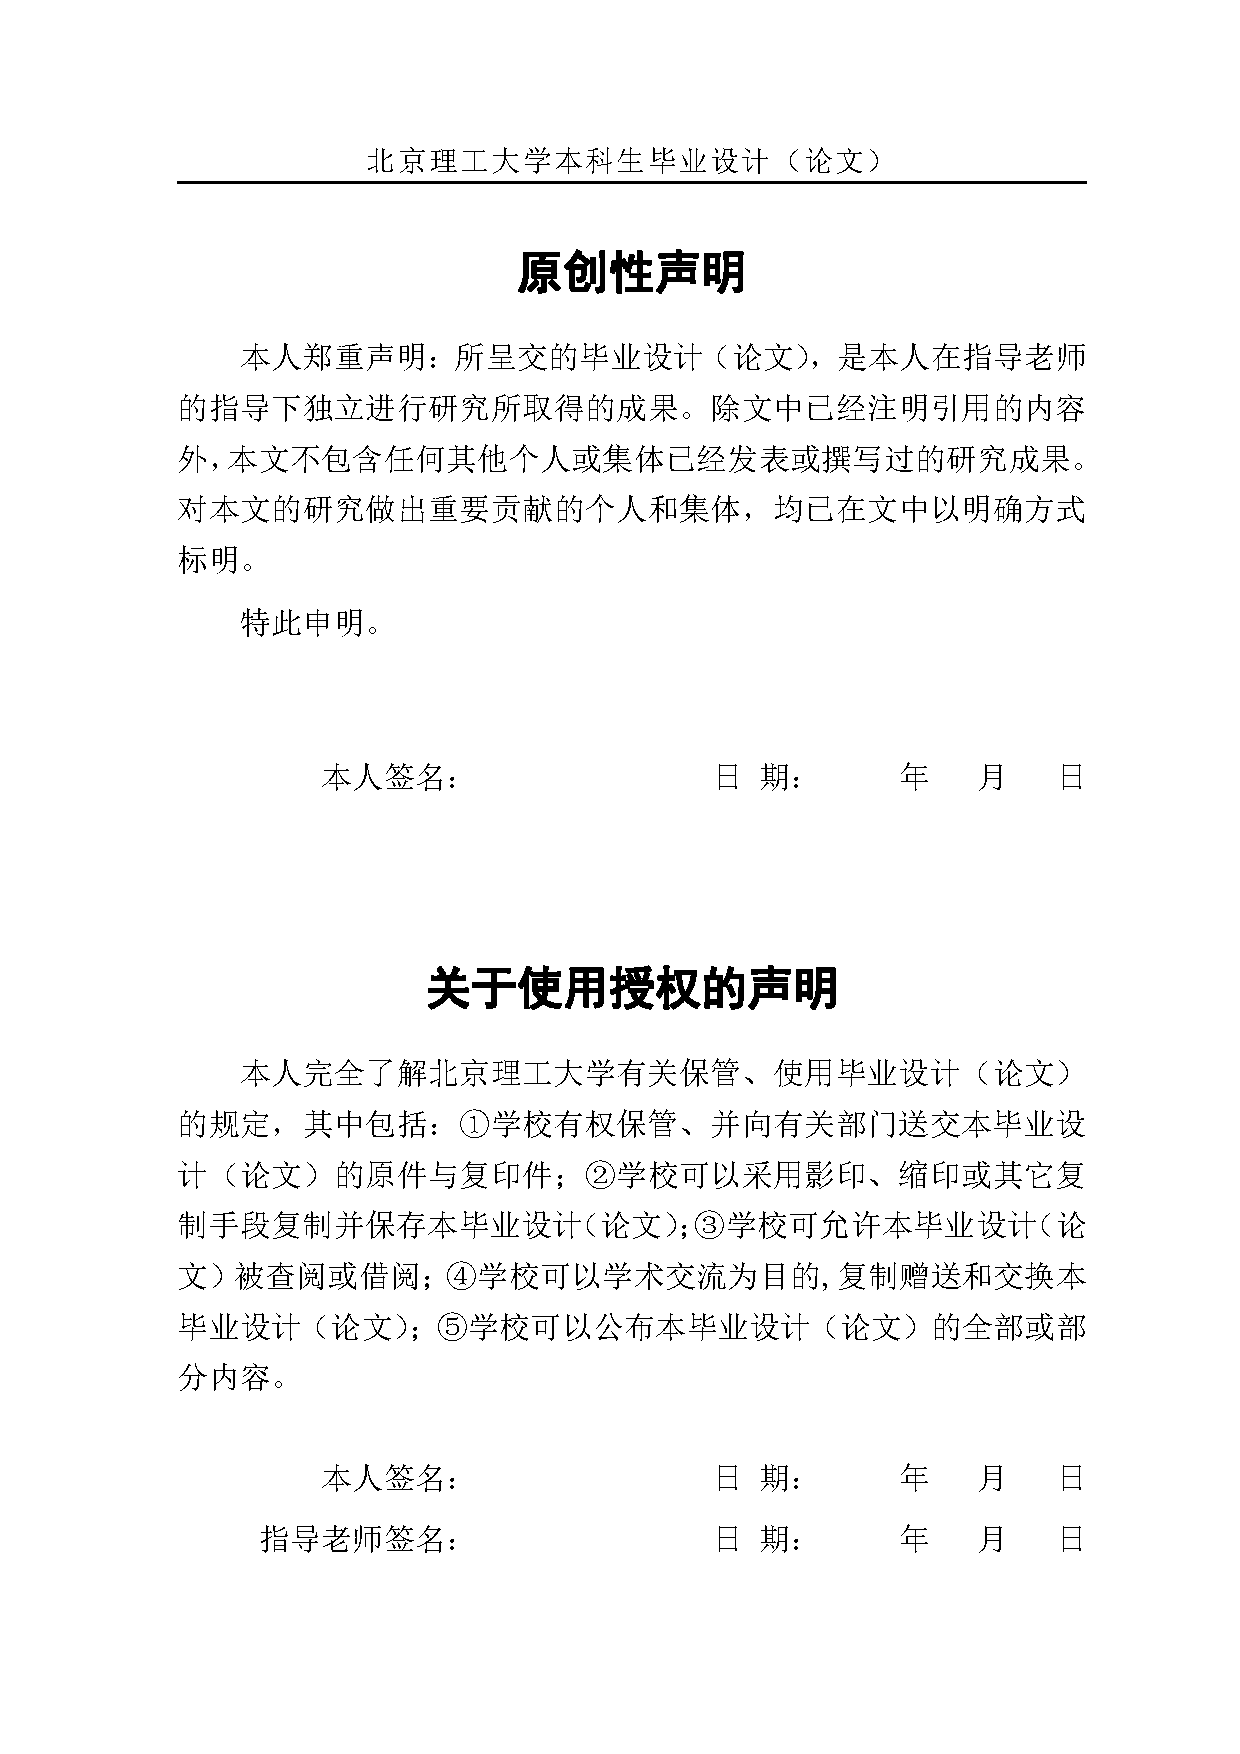
\includepdf{misc/1_originality.pdf}
\newpage
%%%
% The BIThesis Template for Bachelor Graduation Thesis
%
% 北京理工大学毕业设计(论文)原创性声明页 —— 使用 XeLaTeX 编译
%
% Copyright 2020 Spencer Woo
%
% This work may be distributed and/or modified under the
% conditions of the LaTeX Project Public License, either version 1.3
% of this license or (at your option) any later version.
% The latest version of this license is in
%   http://www.latex-project.org/lppl.txt
% and version 1.3 or later is part of all distributions of LaTeX
% version 2005/12/01 or later.
%
% This work has the LPPL maintenance status `maintained'.
%
% The Current Maintainer of this work is Spencer Woo.
%
% 如无特殊需要,本页面无需更改

% 原创性声明页无页码页面格式
\fancypagestyle{originality}{
  % 页眉高度
  \setlength{\headheight}{20pt}

  % 页眉和页脚(页码)的格式设定
  \fancyhf{}
  \fancyhead[C]{\zihao{4}\ziju{0.08}\songti{北京理工大学本科生毕业设计(论文)}}

  % 页眉分割线稍微粗一些
  \renewcommand{\headrulewidth}{0.6pt}
}

\pagestyle{originality}
\topskip=0pt

% 圆形数字编号定义
\newcommand{\circled}[2][]{\tikz[baseline=(char.base)]
  {\node[shape = circle, draw, inner sep = 1pt]
  (char) {\phantom{\ifblank{#1}{#2}{#1}}};
  \node at (char.center) {\makebox[0pt][c]{#2}};}}
\robustify{\circled}

% 设置行间距
\setlength{\parskip}{0.4em}
\renewcommand{\baselinestretch}{1.41}

% 顶部空白
\vspace*{-6mm}

% 原创性声明部分
\begin{center}
  \heiti\zihao{2}\textbf{原创性声明}
\end{center}

% 本部分字号为小三
\zihao{-3}

本人郑重声明:所呈交的毕业设计(论文),是本人在指导老师的指导下独立进行研究所取得的成果。除文中已经注明引用的内容外,本文不包含任何其他个人或集体已经发表或撰写过的研究成果。对本文的研究做出重要贡献的个人和集体,均已在文中以明确方式标明。

特此申明。

\vspace{13mm}

\begin{flushright}
  本人签名:\hspace{40mm}日\hspace{2.5mm}期:\hspace{13mm}年\hspace{8mm}月\hspace{8mm}日
\end{flushright}

\vspace{17mm}

% 使用授权声明部分
\begin{center}
  \heiti\zihao{2}\textbf{关于使用授权的声明}
\end{center}

本人完全了解北京理工大学有关保管、使用毕业设计(论文)的规定,其中包括:\circled{1}学校有权保管、并向有关部门送交本毕业设计(论文)的原件与复印件;\circled{2}学校可以采用影印、缩印或其它复制手段复制并保存本毕业设计(论文);\circled{3}学校可允许本毕业设计(论文)被查阅或借阅;\circled{4}学校可以学术交流为目的,复制赠送和交换本毕业设计(论文);\circled{5}学校可以公布本毕业设计(论文)的全部或部分内容。

\vspace*{1mm}

\begin{flushright}
  \begin{spacing}{1.65}
    \zihao{-3}
    本人签名:\hspace{40mm}日\hspace{2.5mm}期:\hspace{13mm}年\hspace{8mm}月\hspace{8mm}日\\
    指导老师签名:\hspace{40mm}日\hspace{2.5mm}期:\hspace{13mm}年\hspace{8mm}月\hspace{8mm}日
  \end{spacing}
\end{flushright}

\newpage

% 摘要:在摘要相应的 TeX 文件处进行摘要部分的撰写
%%
% The BIThesis Template for Bachelor Graduation Thesis
%
% 北京理工大学毕业设计(论文)中英文摘要 —— 使用 XeLaTeX 编译
%
% Copyright 2020 Spencer Woo
%
% This work may be distributed and/or modified under the
% conditions of the LaTeX Project Public License, either version 1.3
% of this license or (at your option) any later version.
% The latest version of this license is in
%   http://www.latex-project.org/lppl.txt
% and version 1.3 or later is part of all distributions of LaTeX
% version 2005/12/01 or later.
%
% This work has the LPPL maintenance status maintained'.
%
% The Current Maintainer of this work is Spencer Woo.

% 中英文摘要章节
\zihao{-4}
\vspace*{-11mm}

\begin{center}
  \heiti\zihao{-2}\textbf{\thesisTitle}
\end{center}

\vspace*{2mm}

{\let\clearpage\relax \chapter*{\textmd{摘~~~~要}}}
\addcontentsline{toc}{chapter}{摘~~~~要}
\setcounter{page}{1}

\vspace*{1mm}

\setstretch{1.53}
\setlength{\parskip}{0em}

% 中文摘要正文从这里开始
车载自组网是在交通参与者中构建点对点(ad-hoc)开方式网络,提供去中心化、自组织的数据传输服务。目前,区块链的应用越来越广,车载自组网与区块链结合也逐渐变多,利用区块链去中心化、不可篡改等特性,车载自组网可以实现更加可靠的信息传输与交互,但由于车载自组网的移动性以及与地理位置信息紧密结合等特性,导致传统区块链并不能很好的应用于车载自组网上。另外,车载自组网的大量应用都与地理位置信息密切相关,而数据来源于开放的互联网平台,存在被篡改的风险。针对上述两个问题,本文对区块链结构进行相关调研,并对树状区块链进行介绍和复现,同时完成基于该区块链的地图存储和展现。

首先,本文实现了基于GeoHash编码的地图存储与展现,通过智能合约存储地图数据,前端通过web3请求合约数据,最终通过GeoHashTile对地图数据进行呈现,  其中地图数据完全转换为GeoHash编码的GeoJson格式,完成了对传统地图经纬度数据的替换,充分利用了区块链特性保证地图数据的安全性、可塑性以及网络中的同步性。

其次,本文中对树状区块链的相关工作进行了复现,并在此基础上完成基于GeoHash编码的地图存储和展现的部署,并利用李玮琪的车辆位置验证与信誉评估系统验证了树状区块链的正确性,同时对树状区块链存储效率进行了分析。

\vspace{4ex}\noindent\textbf{\heiti 关键词:车载自组网;区块链结构;地图存储与展现;GeoHash编码}
\newpage

% 英文摘要章节
\vspace*{-2mm}

\begin{spacing}{0.95}
  \centering
  \heiti\zihao{3}\textbf{\thesisTitleEN}
\end{spacing}

\vspace*{5mm}

{\let\clearpage\relax \chapter*{
  \zihao{-3}\textmd{Abstract}\vskip -3bp}}
\addcontentsline{toc}{chapter}{Abstract}
\setcounter{page}{2}

\setstretch{1.53}
\setlength{\parskip}{0em}

% 英文摘要正文从这里开始
The vehicular Ad-hoc Networks(VANETs) is to construct an ad-hoc open mode network in traffic participation to provide decentralized and self-organized data transmission services. Currently, the application of blockchain is becoming more and more widespread, and the combination of VANETs and blockchains has gradually increased. Using the characteristics of blockchain decentralization and uncorrectable changes, VANETs can achieve more reliable information. Transmission and interaction, but due to the mobility of the VANETs and its close integration with location information, the traditional blockchain chain cannot be well embedded in the VANETs. In addition, a large number of applications of the VANETs are related to location information, and the open Internet platform for data changes has the risk of being tampered with. In response to the above two problems, the relevant research on the structure of the blockchain chain is carried out, the tree-like blockchain chain is introduced and reproduced again, and the map storage and display based on the blockchain is completed at the same time.

First of all, this article realizes the storage and display of the map based on GeoHash encoding. The map data is stored through the smart contract. The front end requests the contract data through web3. Finally, the map data is presented through GeoHashTile. The map data is completely converted to the GeoJson format of GeoHash encoding. It replaces the traditional map latitude and longitude data, and makes full use of the characteristics of the blockchain to ensure the security, plasticity and synchronization of the map data.

Secondly, this article reproduces the related work of the tree block chain, and on this basis, completes the deployment of the storage and display of the map based on GeoHash encoding, and uses the vehicle location verification and reputation evaluation system of Li Weiqi to verify the tree. The correctness of the blockchain and the storage efficiency of the tree-shaped blockchain are also analyzed.

\vspace{3ex}\noindent\textbf{Key Words: VANET; Blockchain structure; Map storage and display ;GeoHash}
\newpage

% 目录:如无特殊需要,本部分无需改动
%%
% The BIThesis Template for Bachelor Graduation Thesis
%
% 北京理工大学毕业设计(论文)目录 —— 使用 XeLaTeX 编译
%
% Copyright 2020 Spencer Woo
%
% This work may be distributed and/or modified under the
% conditions of the LaTeX Project Public License, either version 1.3
% of this license or (at your option) any later version.
% The latest version of this license is in
%   http://www.latex-project.org/lppl.txt
% and version 1.3 or later is part of all distributions of LaTeX
% version 2005/12/01 or later.
%
% This work has the LPPL maintenance status `maintained'.
%
% The Current Maintainer of this work is Spencer Woo.
%
% 如无特殊需要,本页面无需更改

% 目录开始

% 调整目录行间距
\renewcommand{\baselinestretch}{1.35}
% 目录
\tableofcontents
\newpage


% 正文开始
\mainmatter
% 正文 22 磅的行距
\setlength{\parskip}{0em}
\renewcommand{\baselinestretch}{1.53}
% 修复脚注出现跨页的问题
\interfootnotelinepenalty=10000

% 第一章
%%
% The BIThesis Template for Bachelor Graduation Thesis
%
% 北京理工大学毕业设计(论文)第一章节 —— 使用 XeLaTeX 编译
%
% Copyright 2020 Spencer Woo
%
% This work may be distributed and/or modified under the
% conditions of the LaTeX Project Public License, either version 1.3
% of this license or (at your option) any later version.
% The latest version of this license is in
% http://www.latex-project.org/lppl.txt
% and version 1.3 or later is part of all distributions of LaTeX
% version 2005/12/01 or later.
%
% This work has the LPPL maintenance status maintained'.
%
% The Current Maintainer of this work is Spencer Woo.
%
% 第一章节

\chapter{引言}

\section{课题背景}
% 这里插入一个参考文献,仅作参考
随着智能车的发展与普及,车辆间的交互将变得必不可少,为了营造更加安全高效的车辆交通环境,需要建立车辆间以及车辆与路侧节点的特殊自组网,也就是所谓的“车联网”。在“车联网”中,一大主要应用技术就是车载自组网。车载自组网,是车辆或者路侧节点以自组织的形式构成的多跳网络,为了进行车辆间或车辆与路侧节点间的数据交互\cite{朱雪田20195g}。基于车载自组网,交通参与者之间可以相互通信,形成移动Ad-Hoc网络,并提供去中心化、自组织的数据传输服务\cite{sakiz2017survey}。

区块链最初是作为比特币的基础技术而开发的,它以其创建运行在数百万种设备上的庞大的,全球分布的分类账的能力而迅速成名,该分类账能够记录任何有价值的东西。区块链本质上是一种数字的,分布式的交易分类账,在网络的每台成员计算机上维护着相同的副本。各方都可以查看以前的条目并记录新条目。区块链以轻松、自动化和分散的方式记录的能力引起了各类初创公司和金融服务行业的兴趣,它们正在与多个领域进行融合。\cite{oparah3ways,kar2016estonian}。随着区块链技术的发展与普及,从其活跃的金融市场起,其高度重要性逐渐吸引了不同部门的组织的关注,从移动支付解决方案到医疗保健应用,Blockchain导致了成千上万的新工作岗位和新创业公司的发展\cite{dorri2017blockchain}。

目前,区块链与物联网领域结合的愈发紧密\cite{袁勇2016区块链技术发展现状与展望},区块链上部署相关合约,可以实现无需第三方见证的可信交易,并能够以相同的确定性实现相同的功能,区块链自身具有去中心化、分布式特性,这与车载自组网特性相符,将区块链技术与车载自组网结合起来,能够有效利用区块链的不可篡改性以及可追溯性等特性,解决车载自组网中车辆节点验证问题。

然而,车载自组网中存在很多问题,如车辆节点具备移动特性、车辆网络拓扑结构不断变化,同时,车载自组网中的应用对网络稳定性要求较高,传统的区块链结构已经不能满足上述需求\cite{liu2019kalman}。传统区块链是单链的链式结构,要求所有节点必须存在于同一区块链中,大量的车辆节点将会对区块链存储等问题造成极大影响,而且,传统区块链并没有直接与位置信息联系起来,不满足车辆节点的移动特性。因此,考虑在区块链中增添位置信息,更改传统区块链单链结构,增强区块链对车载自组网的适用性,才能扩展区块链在车载自组网中的应用场景。基于车载自组网的路况查询、事故预警等应用与位置信息联系紧密,攻击者可以伪造地图信息欺骗达到利己的目的,因此,考虑利用区块链特性,将地图信息存储至区块链上,方便多车辆协作,防止数据篡改,为位置信息等提供安全性保障\cite{yang2019maritime}。

\section{相关调研}
\subsection{区块链与智能合约}
区块链是一个共享的不可更改的总账,它用于记录交易、跟踪资产以及建立信任\cite{王震2019面向大数据应用的区块链解决方案综述}。这些资产可以是有形的(房屋,汽车,现金,土地等)或者无形的(知识产权,专利,版权,品牌等)。几乎所有有价值的东西都可以在区块链网络上进行跟踪和交易,从而降低了风险并削减了所有相关成本。交易业务依靠信息,收到的越快、越准确,就会越好。区块链是传递该信息的理想选择,因为它可以提供在不可更改的总账中的即时、共享且完全透明的信息,这类信息同时具备一定的安全性,只能由获得许可的网络成员访问。另外,区块链网络也可以跟踪订单、付款、账户、生产等等。而且因为成员之间可以共享信息,所以成员可以查看到交易端到端的所有细节,从而带来更好的效率。

区块链有三个关键要素,分布式分类账技术、不可篡改以及智能合约。分布式分类账技术是指所有网络参与者都可以访问分布式分类账以及不可变的交易记录,且所有交易仅记录一次,从而消除传统业务网络中大量的重复工作和数据。不可篡改是指,区块链将交易记录到共享的分类账上后无法被篡改,如果交易中包含错误,则必须添加新交易来撤销该错误。

智能合约是存储在区块链上的程序,可以在满足预定条件的情况下运行,它们通常是自动执行的脚本,以便所有参与者无需任何中介机构的参与就可以立即结果,极大保证安全性。智能合约代码语句十分简单,当预定条件已经得到满足并完成验证时,区块链网络将执行对应动作,比如释放资金,发出凭证等,然后交易完成时更新区块链。由智能合约完成的交易也是无法更改的,只有获得许可的参与者才能看到结果。本文的课题是基于以太坊平台来部署智能合约,从而进行相关研究。

\subsection{地理数据表示}
随着移动用户的剧增,交互式信息地图服务需求正在逐渐增多,矢量数据地图正在兴起。在矢量地图数据中,矢量数据可以在所有放缩水平下以不同的颜色正确显示和区分特征,使地图展现更加丰富\cite{zhou2016virtual}。目前矢量地图主要利用Web Map Tile Service(WMTS)框架\cite{garcia2013ols},它可以解决矢量数据分布不均和传输延迟长的问题,在此框架中,地图矢量数据需要被划分为图块,然后根据客户端的请求返回对应图块数据给客户端,通过它们各自的坐标在客户端重新组合,所以矢量数据的编码方式是影响其传输性能和可用性的关键因素。

XML和JSON是web应用程序中常用的两种矢量数据编码方法\cite{wang2011improving}。XML(可扩展标记语言)是一种标记语言,用作Internet信息交换的标准\cite{braysperberg}。它具有良好的语义和可扩展性,并且可以灵活地表示数据,但由于XML使用重量级语法,因此会导致其格式复杂且大小较大,不利于上述地图数据传输。JSON是一种易于读写的轻量级数据表示格式,GeoJson是其中一种轻量级的数据表示方法,用于编码各类地理数据结构,可用于简单表示地理信息\cite{li2015performance}。

传统的矢量地图如Google Maps\cite{kahle2013ggmap},采用二维数据经纬度来表示地理信息,这是一种球面坐标系统。Geohash是一种新型的地址编码方式,它使用Base32编码成一维的字符串代替二维的经纬度数据。与Google Maps经纬度编码相比,GeoHash将二维空间查询转换为一维字符串匹配,利用此优势,GeoHash编码可以实现时间复杂度为O(1)快速查询\cite{liu2014geohash}。与Bing Maps\cite{teslya2014web}相比,GeoHash编码使用Base32编码方法,同一前缀有32个不同子序列,而使用Base4的Bing Maps同一前缀下只有4个子序列。当前,如Google Maps等主流地图产品采用经纬度表示地理数据坐标位置,而索引则采用另一种方法,GeoHash编码可以将二者结合起来,根据编码长度的不同,GeoHash可以同时表示图块的索引范围和坐标,从而可以实现统一编码。同时,GeoHash在编码保留了相对地理位置信息,位数较长的GeoHash编码一定位于对应前缀GeoHash编码所对应的区域中,可以很好的解决区域与具体信息绑定问题。

本文将GeoHash编码用于地图存储与展现上,完全替换传统地图的经纬度数据表示形式,方便了区域信息绑定和查询。

\subsection{区块链结构}
传统区块链技术基于区块,整个网络同时只有一条单链,基于PoW共识机制出块无法并发执行,无法满足车载自组网对高并发操作和网络稳定性的需求,传统区块链也不具备移动性,无法与地理位置信息进行绑定,不能有效利用车载网中地理信息的区域化特性。另外,传统区块链的单链结构,要求所有节点必须在同一区块链中,这将会导致节点数目和数据量过大,不满足车载自组网中车辆节点的移动特性,且一旦出现网络分区,就会对整个区块链产生很大影响。目前采用分片技术更改原始单链的链式结构是解决上述问题的主流方法\cite{global2020}。当前也有多链结构的相关工作。

根据多链结构是否改变底层区块链结构可分为应用多链和结构多链。应用多链,即在应用层面建立不同功能的多个区块链,没有修改底层区块链结构。结构多链,即根据需求对区块链底层结构进行调整的多链结构。
\subsubsection{应用多链}
Shrestha等人\cite{shrestha2019regional}研究了区域区块链在车载自组网中的应用,它是一个由物理边界区域内的节点共享的区块链。如果将区域区块链用于地理有限的区域,由于较小的传播延迟,可以极大减少端到端的消息延迟,提高区块链中节点交易效率,从理论上说,可以将整个区块链分为多个区域区块链,但该文仅从一个区域区块链内部进行了相关研究,并没有设计跨区域和跨链交易的相关内容。

Hirtan等人\cite{hirtan2019blockchain}提出了一种给予隐私保护的医疗保健系统,包含专用链和公用链两种区块链模型。专用链,即侧链,用于保存有关患者的真实身份信息;公用链,即主链,用于存储有关患者健康的信息以及标有临时ID的数据,从而实现了隐私数据保护和可用数据公开访问。通过特定节点掌握患者临时ID和真实身份的关联,来实现两个区块链数据的传递。

Ocha等人\cite{sestrem2020cost}提出了一种使用侧链使智能电网具有可扩展性和适应性的区块链架构,将开放式智能电网协议(OSGP)集成三个区块链中,分别为BlockPRI、BlockSEC和BlockTST。其中,BlockPRI是用于存储每个用户的隐私,BlockSEC存储用户的数据,BlockTST管理和验证有关消费者-消费者和消费者-公司之间的能源贸易的信息。每个区块链对应一个功能,从整体上保证智能电网网络的隐私性和安全性。

\subsubsection{结构多链}
结构多链是根据需求对区块链底层结构进行调整的多链结构,根据其组成特点,结构多链又可以分为并发多链和层次多链。并发多链结构扁平,各个子链可以根据需求负责相同或者不同的功能,相互之间地位平等。而层次多链属于多层级结构,至少具备上下层级关系的子链结构,各个层级负责的功能不同,地位也不同。
\paragraph{并发多链}
Youngjune等人\cite{parkmonoxide}提出异步共识区域,该区域在不影响分散性或安全性的前提下线性扩展了区块链系统。通过建立多个独立并行的单链共识区域来构成并发多链的区块链结构。各个共识组地位平等,大部分交易只在组内完成。分组按指定规则命名,跨组交易采用异步方式将中继事务发送到目标区域,而不是整个网络,减轻了网络负载。此外,为了确保每个区域中的有效采矿能力与整个网络处于同一水平,采用了Chu-ko-nu的改进PoW挖矿方式,这也同时保证了分组抵御攻击的能力。但其共识组分区方法没有考虑实际地理位置信息,不适用于车载自组网。

Zamani等人 \cite{zamani2018rapidchain} 提出了基于分片的公共区块链协议,它将节点划分为多个较小的称为委员会的节点组,节点组在不相交的交易块上并行操作,并维护不相交的独立账本,也就是分片,分片由每个成员以区块链的形式存储。为了解决节点频繁移入移出对网络造成的映像,将委员会将分为活跃和不活跃两个分类,节点创建后,第一次进入委员会需要加入活跃类,再次进入或转移时需要加入不活跃类。RapidChain对分片和跨片交易处理,委员会重组,节点移动都有较好的处理,但也存在一些不足。委员会内节点数量固定,缺少灵活性;委员会构建和重构时没有考虑地理因素,增加了更新时间,不适用于车载自组网。

Feng X等人 \cite{feng2019pruneable} 改进的Rollerchain中利用分片技术和PBFT(拜占庭式容错)算法提出了一种基于可分片的区块链协议(PSRB)。PSRB协议采用分片技术,使得PoW协商机制能够通过特定的社区分配规则和网络的分片功能实现事务的并发管理。社区分配规则为每个节点计算PoW难题,然后根据其nonce分配给某个社区。与现有的区块链协议不同,PSRB协议在每个节点和主链只存储区块头链和部分区块时,保证了系统的安全性,避免了协议的体积膨胀和容量膨胀问题。由于nonce计算的随机性,会出现社区内节点数目差别过大的问题,该方法没有说明对节点处理的方法,且没有结合地理因素,也不适用于车载自组网。

\paragraph{层次多链}
Byung等人 \cite{jo2018hybrid} 将物联网与基于区块链的智能合约相结合,用于结构健康监视(SHM),定义新颖,高效,可扩展和安全的分布式网络,增强运营安全性。该在这个区块链物联网网络中,通过将本地集中和全球分散的分布分为核心和边缘网络,激活了本地集中和全球分散分布的特征,并提供了本地数据库的原始数据存储和核心区块链网络的结构事件存储两种类型的存储。边缘节点充当查询实时响应的集中式服务器,并提供低延迟和带宽使用率,核心网络由具有高存储容量的miner节点组成,负责生成新块、验证工作证明(PoW),并包含用于自主决策的智能合约,这种划分提高了系统的效率和可伸缩性且可以有效地模拟结构的自主监测和控制,但核心网络十分庞大是主要问题 。核心网络的庞大影响移动节点的交易效率,且该区块链也没有考虑地理因素,不适用于车载自组网。

Liu等人 \cite{liu2019mathsf} 为解决部署区块链和处理事务负担过大,提出了LightChain的轻量级区块链系统,该系统由API层,LightChain层, 缓存层和存储层等4层框架构成。API层用来读写本地数据和构造区块链交易;LightChain层通过数字签名验证和附件验证用来验证交易的有效性和完整性;缓存层是为了加速对调用的响应而设计的,它包含本地操作、未验证的块和有用的块;存储层通常由资源丰富的设备提供服务,为上层提供持久存储服务。该结构,解决了部署区块链和处理事务的过重负担,但由于其并没有考虑地理因素,不能很好的应用于车载自组网,但其缓存机制,可以参考,用于加速对调用的响应。

Pajooh等人\cite{honar2021multi}提出了一种多层区块链安全模型来保护物联网网络,同时利用群集的概念来简化多层架构,通过使用模拟退火和遗传算法相结合的混合进化算法来定义物联网K-未知簇,选择的群集头负责本地身份验证和授权,增强了网络认证机制的安全性,显示出更适合的平衡网络延迟和吞吐量。

Chao Q等人\cite{qu2018blockchain}提出了一个具有分层、交叉和自组织区块链结构(BCS)的框架,以建立物联网和区块链之间的关系来验证设备可信度。该工作主要包括三个部分:第一部分,上层区块链节点管理一个下层的区块链节点,不同的区块链网络构成一个层次关系;第二部分,底层的寄存器数据依次传输到上层区块链节点,并途经区块链同样记录数据,第三部分,沿着源设备到目标设备形成验证链。

Mbarek等人\cite{mbarek2019mbs}提出了一个多级区块链框架,以增强物联网应用中的隐私和数据安全。多层次模型侧重于提高响应时间和资源利用率。方案中定义了移动代理来执行哈希函数、实现加密、部署聚合和解密。移动代理在区块链和物联网之间传输,以完成所需的任务。该多层次框架由微观层次(物联网设备层次)、中观层次区块链(物联网的簇头层次)和宏观层次区块链(平台层次或物联网的最高层次)等三层次组成。

Oktian等人\cite{oktian2020hierarchical}提出了一个可扩展的物联网双层分层区块链体系结构。第一层是基于实用拜占庭容错(PBFT)共识来处理高吞吐量的核心引擎,第二层分别由支付引擎、计算引擎和存储引擎组成,用来管理底层的从属引擎(子引擎)。该作者将这些子引擎的多个实例部署到尽可能多的位置,并尽量靠近物联网设备所在的物联网域,以应对大量节点。此外,为了进一步扩展所提出的体系结构的可伸缩性,该作者还在核心引擎上提供了额外的可伸缩性特性,如请求聚合、请求优先级以及子引擎并行性。

\paragraph{智能合约多链}
Ochôa等人\cite{sestrem2020cost}提出了侧链结构,由BlockPRI、BlockSEC、BlockTST三个不同的区块链,使用了三个区块链来确保系统的隐私性,安全性和信任性。BlockPRI存储每个用户的隐私首选项。 BlockSEC存储用户的数据。最后,BlockTST管理并验证有关消费者-生产者与消费者-公司之间的能源贸易的信息。为了保证区块链之间的通信,需要通过智能合约维护多链数据一致性。

\subsection{论文的研究内容及贡献}
本文将传统地图的经纬度数据完成转变为GeoHash编码,并将存储至区块链上,并通过GeoHashTile前端将地图数据进行呈现,利用区块链不可篡改特性,极大的保护了车载自组网中地图数据安全。另外,由于全局同步与共识速度的限制,传统区块链发挥车载自组网的高动态性与地理位置相关等特性。为了解决上述问题,本文还对区块链多链结构进行了相关调研,同时介绍了与地理信息相关的树状区块链并对其进行了复现,同时将地图存储与展现应用于树状区块链上,验证了树状区块链的可行性与正确性,最后对树状区块链进行了一些测试工作。

(1) 准备阶段,通过复现前人相关工作,熟悉了区块链的相关知识。在目前最新的开发和测试环境下,对其工作进行复现,途中遇到很多问题,编写了相关文档,为后人提供帮助;

(2)  成功将地图数据以GeoHash编码格式存储至传统区块链上,并实现区域信息绑定,快速查询指定区域地图数据;

(3) 成功将存储的地图数据以GeoHashTile前端展现,并成功运行车辆位置验证及信誉评估系统,完成了对地图数据正确性的验证;

(4) 将上述工作全部移植到树状区块链上,成功验证树状区块链的正确性;

(5) 对树状区块链进行了相关测试工作。
% 在这里添加第二章、第三章……TeX 文件的引用
%%
% The BIThesis Template for Bachelor Graduation Thesis
%
% 北京理工大学毕业设计(论文)第一章节 —— 使用 XeLaTeX 编译
%
% Copyright 2020 Spencer Woo
%
% This work may be distributed and/or modified under the
% conditions of the LaTeX Project Public License, either version 1.3
% of this license or (at your option) any later version.
% The latest version of this license is in
%   http://www.latex-project.org/lppl.txt
% and version 1.3 or later is part of all distributions of LaTeX
% version 2005/12/01 or later.
%
% This work has the LPPL maintenance status maintained'.
%
% The Current Maintainer of this work is Spencer Woo.
%
% 第二章节
\chapter{树状区块链}
本章中,介绍了树状区块链的应用场景,对其相关工作进行了简单调研,并详细描述其具体研究内容与原理,最终解决了树状区块链中合约部署与调用问题,完成了树状区块链的复现。
\section{背景介绍}
车联网是指车辆与车辆、行人、基础设施以及因特网的通讯的大型通信网络概念。在车联网中,主要有蜂窝移动网络和车载自组网两种不同的接入方式,车载自组网具备低成本、低时延以及地理位置天然联系的特性,是对蜂窝数据的重要补充,在道路安全等应用提供了重要支持\cite{klapez2020application}。

近年来,智能汽车的车辆数量变多,车辆与车辆、基础设施的交互也变得越来越多,势必导致数据安全、隐私、信任等相关安全性问题\cite{汤立波2019车联网产业融合发展趋势,VN2020}。区块链作为一种新型的互联网模式,具备去中心化、不可篡改、可追溯等特点,与车联网的联系愈发紧密,但实际应用上还是存在许多问题\cite{mollah2020blockchain}。其中主要包括两个问题,首先,区块链技术通常要求可靠的网络接入,存在网络覆盖以及基础设施成本问题 ,而车载自组网的接入方式由网络高动态性引发的网络不稳定对区块链的应用造成了极大的挑战。其次,车载自组网中的信息通常与地理信息天然绑定,而传统区块链并不具备此特性。因此,研究地理位置与区块链的融合就是为上述地理区域问题提供一种可能的解决方案。

\section{相关工作}
车联网与区块链的应用愈发紧密,然而,传统区块链的特点不能满足车载自组网的特性。一方面,传统区块链吞吐量较小、出块速度慢,需要改善它的结构来提升可扩展性;另一方面,传统区块链与真实世界的联系较弱,而车联网与地理信息有天然联系并且紧密相关,因此传统区块链结构不能很好适应车联网\cite{wagner2018cyber}。

就目前来说,一种主流的方案是将区块链的单链结构改良位多链结构\cite{global2020}。根据多链结构的构成方式的不同,可以将相关工作分为三类:并发多链\cite{parkmonoxide,zamani2018rapidchain,feng2019pruneable},层次多链 \cite{jo2018hybrid,liu2019mathsf,honar2021multi,qu2018blockchain,sharma2018blockchain,mbarek2019mbs,oktian2020hierarchical},智能合约多链\cite{sestrem2020cost}。并发多链存在多条子链,每条子链对应一个独立的功能模块,主链只负责维护多条子链的数据一致性;层次多链中,区块以层次化的结构组成区块链,各个层级具有上下从属关系;智能合约多链与并发多链结构类似,区别在于智能合约多链不修改区块链数据结构,通过智能合约维护多链数据一致性,存在多链数据同步的效率以及地理信息相关数据的存储以及检索的问题。而将地理位置融合进区块链的数据结构,实现层次化多链,这就是所谓的树状区块链。

\section{研究内容及原理}
由于全局同步与共识速度的限制,传统区块链不能很好的适应车载自组网的高动态性,极大的影响了区块链的效能,并且不能保证车辆与路侧节点的稳定连接,这将会极大影响到区块链共识机制的可用性。车载自组网与地理信息天然相联,并且车辆通常仅需要关注特定区域的信息,而传统区块链记录的交易信息不包含位置,无法根据地理区域查询交易,且传统区块链全局同步的设计会造成网络资源的大量浪费,并且传统区块链只能方便查询某个账户的交易、最新的交易、指定区块内包含的交易,无法高效的查询地理信息相关的数据。

树状区块链的研究就是为了解决上述问题,对区块链的结构进行修改与优化,使其更能适应车载自组网特性。树状区块链是一种基于位置的区块链,首先,根据GeoHash地理编码与地理区域层次关系建立树状结构的区块,同时研究树状结构地理信息相关数据查询速度的优化机制,从而提升区块链在车载自组网中的吞吐量以及与地理信息相关数据的检索速度。

GeoHash是一个能表示任意精度的高效地理编码系统,它使用二分法将指定区域分为网格,每个网格由唯一的编码表示,网络的大小对应的层次不同,编码越长对应的网格越小,层次越低。树状区块链使用GeoHash地理编码作为基本数据编码方式。建立 GeoHash 与区块以及交易的索引,从而依据GeoHash编码直接获取区域交易内容,同时,GeoHash编码可以通过前缀对区域信息进行绑定,因此通过GeoHash编码可以很自然地建立区域层次与子链的联系。

树状区块链主要包括三个部分的工作:更改区块数据结构、区块与节点的层次化分类以及区块的层次化组织。

\begin{enumerate}
 \item 区块链结构 \\
 如图\ref{树状区块链结构变化},树状区块链是基于以太坊的区块链数据结构进行修改的,在其基础上主要新增如下数据结构:\\
 \begin{figure}[!htb]
  \centering
  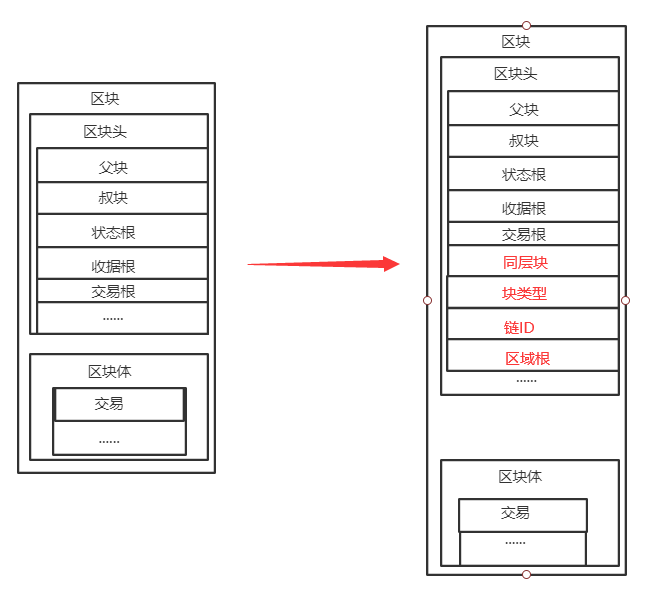
\includegraphics[width=5in]{images/1.png}
  \caption{树状区块链结构变化}\label{树状区块链结构变化} % label 用来在文中索引
\end{figure}

 \begin{enumerate}
  \item 同层块指针:记录与本区块同层次地理区域对应区块的哈希,与父块哈希一同构成树状区块链。
  \item 位置:使用指定长度的 Geohash 编码表示位置,分别在账户状态、交易数据中新增位置信息,增加账户、交易与物理世界的关联。
  \item 区域状态树:以Geohash作为索引构建字典树,存储区域内的四种信息:当前区域内的账户(Account)、交易(TXID)、收据(RPID)以及上层区域状态树根节点列表(URRList)记录所有上层区域状态树的根节点哈希,如图\ref{区域状态树}。
  
  \begin{figure}[!htb]
    \centering
    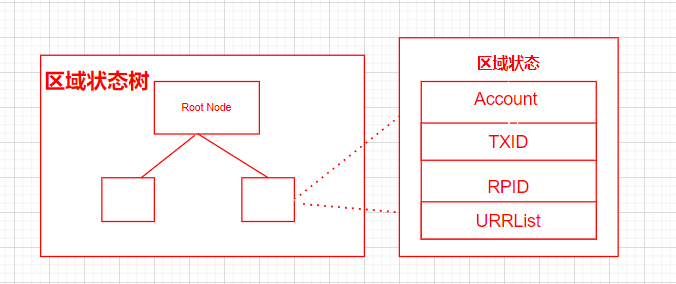
\includegraphics[width=5in]{images/14.png}
    \caption{区域状态树}\label{区域状态树} % label 用来在文中索引
  \end{figure}
  \item 账户位置树:在外部账户的账户状态中以发生交易时的,记录账户发生过的交易所在的区域。可以提供以下功能:根据位置区域,查询该区域内最新交易;查询某个账户在指定区域的交易以及历史交易发生的位置,如图\ref{账户状态树}。
  \begin{figure}[!htb]
    \centering
    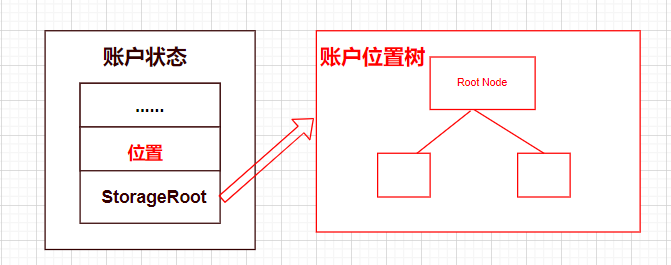
\includegraphics[width=5in]{images/15.png}
    \caption{账户状态树}\label{账户状态树} % label 用来在文中索引
  \end{figure}
 \end{enumerate}
 \item 区块与节点的层次化分类 \\ 为了将区块链划分为树状结构,首先将区块按其特征分为三种:
 \begin{enumerate}
  \item 创世块:区块链的初始区块。
  \item 分支块:根据 Geohash 编码以层次化结构一一对应创建分支区块作为对应区域内子链的头区块,只维护直接下层区域的索引信息,不记录交易信息。
  \item 普通块:地理区域的最小划分对应分支区块的子区块,记录在对应地理区域内发生的交易。
 \end{enumerate}
 其次,将网络节点按照其功能分为三种:
 \begin{enumerate}
  \item 全节点:维护全区块链完整区块数据和全局状态树,部分服务器为全节点。
  \item 区域节点:维护其所在区域内指定层次及以下的所有分支区块与普通区块。每个分支节点负责向上层节点更新汇总当前区域状态并同步所有上层区块链的区域状态树根节点列表。路侧节点与部分服务器为区域节点。
  \item 叶节点:维护所在区域内最下层分支区块以及普通区块。负责局部共识,以及在与区域节点有连接机会时上传缓存信息,并同步所有上层区块链的区域状态树根节点列表。车辆节点为叶节点。
 \end{enumerate}
 \item 区块的层次化组织 \par 
 在树状区块链设计中,只有普通区块会记录实际发生的交易,分支区块提供子区区块链头区块以及索引功能。每个地理区域都有对应一个分支区块和多个普通区块通过父块哈希指针组成的区块链,同层次不同区域多赢的分支区块之间通过同层块指针链接起来。分支区块的层次关系代表地理区域的包含关系,即上层分支区块对应的地理区域包含所有以该区块为父块的下层区块对应的地理区域。
\end{enumerate}

树状区块链与传统区块链相比,融合了地理位置,增加了区块链与真实世界的联系,设计了区块状态树和账户位置树提升与地理信息相关数据的检索速度。

\section{树状区块链的复现}
树状区块链是基于以太坊开发的。通过更改其以太坊底层区块链结构,增添区域状态树以及账户状态树,由go语言编译为新的geth客户端。本小节将对树状区块链所属geth客户端进行编译复现,并以此为基础建立一条基于树状区块链的私有链。

首先,下载源代码,配置go语言环境。从对应代码仓库将源码下载,使用go语言环境直接进行编译,生成最新版的树状区块链的geth客户端。为了方便后续使用,将该geth程序放入/usr/bin中。使用geth version确定geth能够正确使用。

然后,建立树状区块链私有链,创建创世块genesis.json文件,具体内容见附件C。
在同一文件夹下,初始化树状区块链私链:
\begin{center}
  \fbox{
    \parbox{130mm}{
      geth --identity "MyEth" --rpc --rpcaddr 127.0.0.1  --rpcport "8545" --rpccorsdomain "*" --datadir gethdata --port "30303" --nodiscover --rpcapi "eth,net,personal,web3" --networkid 91036 init genesisgtrie.json
    }
  }
\end{center}

在同一文件夹下,启动树状区块链:
\begin{center}
  \fbox{
    \parbox{130mm}{
      geth --identity "MyEth" --rpcaddr 127.0.0.1 --rpc --rpcport "8545" --rpccorsdomain "*" --datadir gethdata --port "30303" --nodiscover --rpcapi "eth,net,personal,web3" --networkid 91036 --allow-insecure-unlock --dev.period 1 console
    }
  }
\end{center}

创建新账户:
\begin{center}
  \fbox{
    \parbox{130mm}{
      personal.newAccount("123456")
    }
  }
\end{center}

输入测试数据,测试树状区块链功能函数:
\begin{center}
  \fbox{
    \parbox{130mm}{
      eth.getPosition(eth.accounts[0]) \# 查看账户位置 \\
      eth.getPosition(eth.accounts[0],1) \# 查询block=1时,accounts[0]的位置 \\
      eth.getStorageAt(eth.accounts[0],2)\# 查询在txtime=2时,accounts[0]的位置 \\
      eth.getAccountByRegion("wx111111111111") \# 根据GeoHash查询账户 \\
      eth.getTxByRegion("wx111111111111")      \# 根据GeoHash查询Tx信息 \\
      eth.getRpByRegion("wx111111111111")      \# 根据GeoHash查询Region信息 
    }
  }
\end{center}

以上内容,如果全部正确运行下来,没有出现报错,则证明复现成功,且树状区块链增添的相关位置信息的功能能够正常运行,至此完成复现。

 \section{树状区块链的合约部署与调用}
  在进行树状区块链合约部署的时候遇到两个问题,首先,与传统区块链不同,部署合约需要添加position和txttime参数,其次,在进行合约调用的时候,合约中的get方法中参数不能为空。

  目前,本文已经解决树状区块链部署问题,下面对其流程进行阐述。
  
  首先,运行私链,然后解锁帐户,合约可以使用truffle工具进行编译,在生成的Build文件夹下找到对应的json文件,获取其中的abi以及bytecode,随即在客户端上运行如下命令:
  \begin{center}
    \fbox{
        \parbox{130mm}{
        abi = JSON.parse('') \\
        bytecode = ""\\
        QualContract = web3.eth.contract(abi);
      }
    }
\end{center}

使用如下命令对部署合约所需要使用的Gas进行评估:
\begin{center}
  \fbox{
      web3.eth.estimateGas({data: bytecode})
  }
\end{center} 

如果在部署时合约对应部分,如果不添加position和txttime参数,树状区块链的私有链将会直接崩溃,所以在部署智能合约时需要增添对应参数,完成合约部署:
\begin{center}
  \fbox{
    \parbox{130mm}{
      Qual = QualContract.new(\{ \\
      from: web3.eth.accounts[0], \\
      data: bytecode, \\
      gas: '800000',\\
      position:"w25111111111113",\\
      txtime:277001\\
 \},function (e, contract)\{\\
      console.log(e, contract);\\
      if(!e)\{\\
          if(!contract.address) \{\\
              console.log("Contract transaction send: TransactionHash: " \par  + contract.transactionHash + " waiting to be mined...");\\
          \} \\else \{\\
              console.log("Contract mined! Address: " + contract.address);\\
              console.log(contract);\\
          \}
      \}
  \});
    }
  }
\end{center}

调用合约,合约调用中send方法也需要增添position和txttime参数,否则树状区块链也会崩溃,调用实例如下:
\begin{center}
  \fbox{
    \parbox{130mm}{
    trafficContract.methods.setSlingePos(userId, locTime[index], latOri, lonOri, latFix, lonFix).send(
    \{from: trafficContractAccount, gas: 500000,position:"w25111111111113",txttime:100\});
    }
  }
\end{center}

由于之前的树状区块链区块中,get方法中参数不能为空,为此,在树状区块链底层代码中get方式处增添缺省值,完成了对此问题的解决。

 \section{小结}
 本章中,首先,介绍了树状区块链的研究内容与原理,树状区块链对区块数据结构、区块与节点的层次化分类以及区块的层次化组织进行了研究,根据GeoHash地图编码与地理区域层次关系建立树状结构的区块,最终达到提升区块链在车载自组网中的应用范围。其次,根据前人相关工作完成了对树状区块链的复现,并解决了智能合约部署与调用的问题,使得树状区块链功能更加完整。
%%
% The BIThesis Template for Bachelor Graduation Thesis
%
% 北京理工大学毕业设计(论文)第一章节 —— 使用 XeLaTeX 编译
%
% Copyright 2020 Spencer Woo
%
% This work may be distributed and/or modified under the
% conditions of the LaTeX Project Public License, either version 1.3
% of this license or (at your option) any later version.
% The latest version of this license is in
%   http://www.latex-project.org/lppl.txt
% and version 1.3 or later is part of all distributions of LaTeX
% version 2005/12/01 or later.
%
% This work has the LPPL maintenance status maintained'.
%
% The Current Maintainer of this work is Spencer Woo.
%
% 第三章节
\chapter{基于GeoHash的地图信息存储}
车辆位置信息和地图信息在路由和安全应用中发挥着重要作用。攻击者可以通过位置欺骗达到利己的目的。利用区块链特性,方便多车辆协作,防止数据篡改,为位置信息等提供安全性保障。在本章中,将介绍如何将地图数据处理为GeoHash编码,并实现区域绑定,最终将其存入区块链上。

\section{相关技术}
\subsection{GeoHash编码}
GeoHash是一种新型的地址编码方式,由 Gustavo Niemeyer 和 G.M. Morton发明\cite{lposition},其具体算法是二分法结合编码的一种地理位置信息算法\cite{liu2014geohash},被广泛应用到地理位置表示中。最开始,以本初子午线、赤道为界,地球可以分为4个部分,设定西经为负,南纬为负,所以地球上的经度范围就是[-180,180],纬度范围就是[-90,90]。经纬度的二进制码也是通过二分来进行确认的,以(116.3639092,39.9662639)为例,经纬度转为二进制编码,GeoHash精度为8,过程如下表\ref{经纬度计算}所示。

\begin{table}[!ht]
  \centering
  \caption{经纬度计算}
  \label{经纬度计算}
  \subcaption*{Table1 经度计算}
  \begin{tabular}{*{5}{>{\centering\arraybackslash}p{3cm}}}
  \hline
         &  经度范围             & 划分区间(0)           & 划分区间(1)            &  116.3639092   \\ \hline
    1    &  (-180,180)         & (-180,0)             & (0,180)              & 1  \\
    2    & 	(0,180)            & (0,90)               & (90,180)             & 1  \\
    3    & 	(90,180)           & (90,135)             & (135,180)            & 0  \\ 
    4    & (90,135)            & (90,112.5)            & (112.5,135)           & 1 \\ 
    5    & (112.5,135)          &	(112.5,123.75)        & 	(123.75,135)        & 0 \\ 
    6    & (112.5,123.75)       & (112.5,118.125)      & (118.125,123.75)      & 0 \\ 
    7    & (112.5,118.125)     & (112.5,115.3125)     & (115.3125,118.125)    & 	1 \\ 
    8    & (115.3125,118.125)	& (115.3125,116.71875) & (116.71875,118.125)	 & 	0 \\ 
    \hline
    \end{tabular}
  \bigskip
  \subcaption*{Table2 纬度计算}
  \begin{tabular}{*{5}{>{\centering\arraybackslash}p{3cm}}}
    \hline
           & 纬度范围    & 划分区间(0)    & 划分区间(1)   &  39.9662639   \\ \hline
    1    & (-90,90)  & 	(-90,0) & (0,90)  & 1  \\
    2   & 	(0,90)  & (0,45)  & (45,90)  & 0  \\
    3 & 	(0,45)  & (0,22.5)  & (22.5,45)  & 1  \\ 
    4    & 	(22.5,45) & 	(22.5,33.75) & (33.75,45) & 1 \\ 
    5    & (33.75,45) &		(33.75,39.375) & (39.375,45) & 1 \\ 
    6    & (39.375,45) & (39.375,42.1875) & (42.1875,45) & 0 \\ 
    7    & (39.375,42.1875) & (39.375,40.78125) & (40.78125,42.1875)	 & 	0 \\ 
    8    & 	(39.375,40.78125)	 & 	(39.375,40.078125) & (40.078125,40.78125)	 & 	0 \\ 
    \hline
    \end{tabular}
\end{table}

将经度和纬度分别转换成一组二进制字符串,然后将经度和纬度的二进制字符串交叉结合成一组新的二进制字符串,新的二进制字符串中对应偶数位的序列是经度序列,对应奇数位的序列是纬度序列,然后将新字符串转为十进制并根据Base32(即数字0-9和字母b-z不包括a,i,l,o的32个字符)进行编码\cite{liu2014geohash},最终实现用一维数据表示二维数据的效果。

Geohash特殊的编码方式,一个GeoHash值对应一个近似矩形的覆盖区域,当位数较少时,它可以表示一块区域的坐标,当位数足够长时,它可以表示地球上某个具体点的坐标,而且,位数短的区域一定包含以此为前缀的地图数据,对地图数据进行区域绑定提供了极大的便利。GeoHash在编码过程中保留了一定的相对地理位置信息,在大部分情况下,GeoHash编码共同前缀越长的区块物理距离越近\cite{lposition}。

传统的地图数据采用经纬度的方法进行存储,不方便实现位置与区域绑定,采用GeoHash字符串存储地图信息可以使所有信息平面化,避免使用树状结构,更方便区域信息绑定,也更适用于Solidity语言特性。同时,根据GeoHash编码规则,一个GeoHash值所代表的区域一定包含以该GeoHash值为前缀的所有元素。

\subsection{区块链}
区块链具有去中心化、分布式、点对点、集体维护等特点,其上交易的不可更改性保证了数据的可靠性,通过编写智能合约,将地图数据存入区块链,可以使得移动端用户获取安全正确的数据,且稳定性更高,更有利于车载终端互连。

\subsection{Web3Js}
前端使用web3js-v1.2.29调用,首先需要Web3.providers.HttpProvider绑定监测IP:
\begin{center}
  \fbox{
    web3Map = new Web3(new Web3.providers.HttpProvider(mapContractServer));
  }
\end{center}

然后使用eth.Contract绑定对应合约,其中mapContractAbi是合约接口,mapContractAddress是合约部署到区块链上的地址:
\begin{center}
  \fbox{
    mapContract = new web3Map.eth.Contract(mapContractAbi,mapContractAddress);	
  }
\end{center}

在与合约进行交易的时候,需要调用methods下的call和send方法,如果是发送交易,需要更改区块链数据则调用send方法:
\begin{center}
  \fbox{
    \parbox{130mm}{
    trafficContract.methods.setSlingePos(userId, locTime[index], latOri, lonOri, latFix, lonFix).send(
    \{from: trafficContractAccount, gas: 500000\});
    }
  }
\end{center}

如果是获取区块链上的数据则使用call方法:
\begin{center}
  \fbox{
    \parbox{130mm}{
      trafficContract.methods.getQuality(userId).call(function(error, result)\{
      \par if(!error) \{
      \par      console(result);
      \par          \} else
      \par    console.error(error);
      \});
    }
    }
\end{center}

\section{实现思路}
\subsection{数据转换}
原始数据为GeoJson的经纬度格式,如下:

(1) 点:
\begin{center}
  \fbox{
    \parbox{130mm}{
      \{"type":"Feature","geometry":\{"type":"Point","coordinates":[116.3639092,\par 39.9662639]\},"properties":\{"highway":"traffic\_signals","name":"name"\par \}\}
    }
  }
\end{center}

(2) 道路:
\begin{center}
  \fbox{
    \parbox{130mm}{
      \{"type":"Feature","geometry":\{"type":"LineString","coordinates":[[\par 116.3894407, 39.9062721],[116.3894463,39.9060115]]\},\par "properties":\{"highway":"primary","name":"广场西侧路",\par "oneway":"yes"\}\}
    }
  }
\end{center}

(3) 建筑物:
\begin{center}
  \fbox{
    \parbox{130mm}{
      \{"type":"Feature","geometry":\{"type":"MultiPolygon","coordinates":[[[[\par 116.390632,39.9165908],[116.3906404,39.9163544],[116.3908015,\par 39.9163577],[116.3909492,39.9163608],[116.3909408,39.9165972],\par [116.3907829,39.9165939],[116.390632,39.9165908]]]]\},"properties":\{ \par "building":"yes","name":"中和殿"\}\}
    }
  }
\end{center}

编写JS脚本将对应坐标数据转化为GeoHash编码:

(1) 点:
\begin{center}
  \fbox{
    \parbox{130mm}{
      \{"type":"Feature","geometry":\{"type":"Point","coordinates":["wx4ergts7ee" \par ]]\},"properties":\{"highway":"traffic\_signals","name":"name"\par \}\}
    }
  }
\end{center}

(2) 道路:
\begin{center}
  \fbox{
    \parbox{130mm}{
      \{"type":"Feature","geometry":\{"type":"LineString","coordinates":[[ \par "wx4g088nys3","wx4g088jqet"]\},"properties":\{"highway":"primary" \par ,"name":"广场西侧路","oneway":"yes"\}\}
    }
  }
\end{center}

(3) 建筑物:
\begin{center}
  \fbox{
    \parbox{130mm}{
      \{"type":"Feature","geometry":\{"type":"MultiPolygon","coordinates":[[[ \par 'wx4g0d94frc','wx4g0d91d7z','wx4g0d91whr','wx4g0d939sy', \par 'wx4g0d9713p','wx4g0d95jb6','wx4g0d94frc']]]\},"properties":\{ \par "building":"yes","name":"中和殿"\}\}
    }
  }
\end{center}

\subsection{绑定方法}
在存储地图时,本文将地图划分为精度较低、范围较广的GeoHash块,并实现对应区域中元素与GeoHash块一一绑定,因此想要请求某一区域的地图信息时,只需要通过该区域对应的GeoHash编码值查找。完整的地图数据主要有三种元素:点,道路,建筑物。

在进行绑定时,点只需要绑定到前缀所代表的区域上,根据GeoHash编码规则,3区域的红色点的GeoHash值一定是红色点的前缀,本课题中,通过直接绑定前缀即可绑定区域,如图\ref{点绑定区域}。
\begin{figure}[!htb]
    \centering
    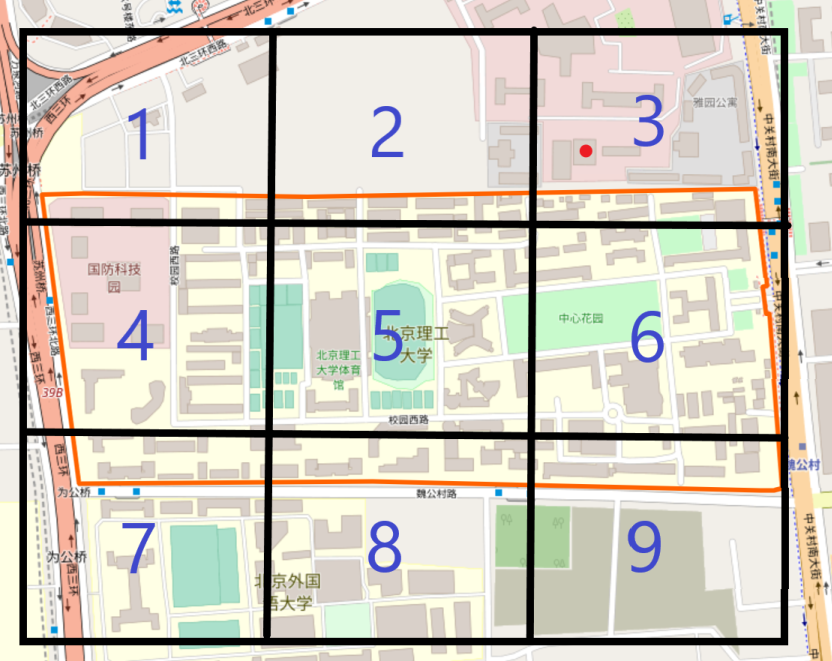
\includegraphics[width=4in]{images/3.png}
    \caption{点绑定区域}\label{点绑定区域} % label 用来在文中索引
\end{figure}

对于道路,地图数据中以矢量的形式出现,取其起点和终点,将其当作一条直线,对于经纬度,0.01°经度代表1000m,0.01°纬度代表1113m,所以通过遍历从起点到终点的经纬度,以0.01°为间隔,划分出对应区域,然后通过前缀判断与路径上的点是否有交叉,从而判断该直线是否在该区域内。如图\ref{道路绑定区域},红色路径经过区域4和区域7,通过上述遍历,可以划分出直线所经过的区域编码,如果该路径存在点在区域4中,则属于区域4,同理,如果存在点在区域7中,则属于区域7。
\begin{figure}[H]
    \centering
    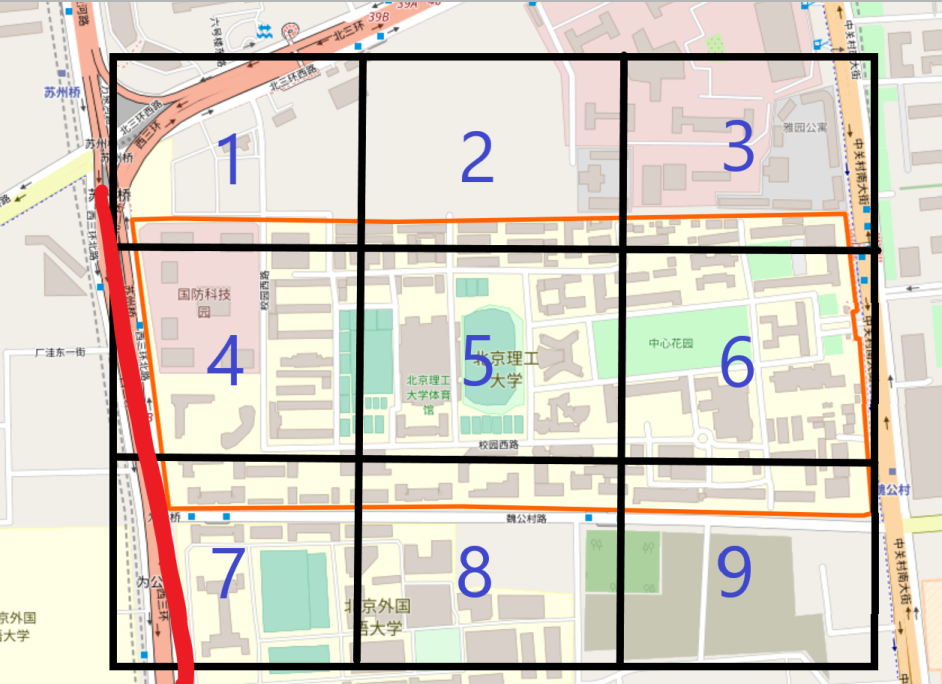
\includegraphics[width=4in]{images/4.png}
    \caption{道路绑定区域}\label{道路绑定区域} % label 用来在文中索引
  \end{figure}

对于建筑物,地图数据中建筑物是多边形数据,且建筑物一般横跨区域不大,所以通过遍历多边形上的点元素,将其绑定到前缀所对应的区域上,即可完成建筑物绑定。如图\ref{建筑物绑定区域},图中中心花园区域横跨两个区域,可通过对应路径前缀进行绑定。
\begin{figure}[H]
    \centering
    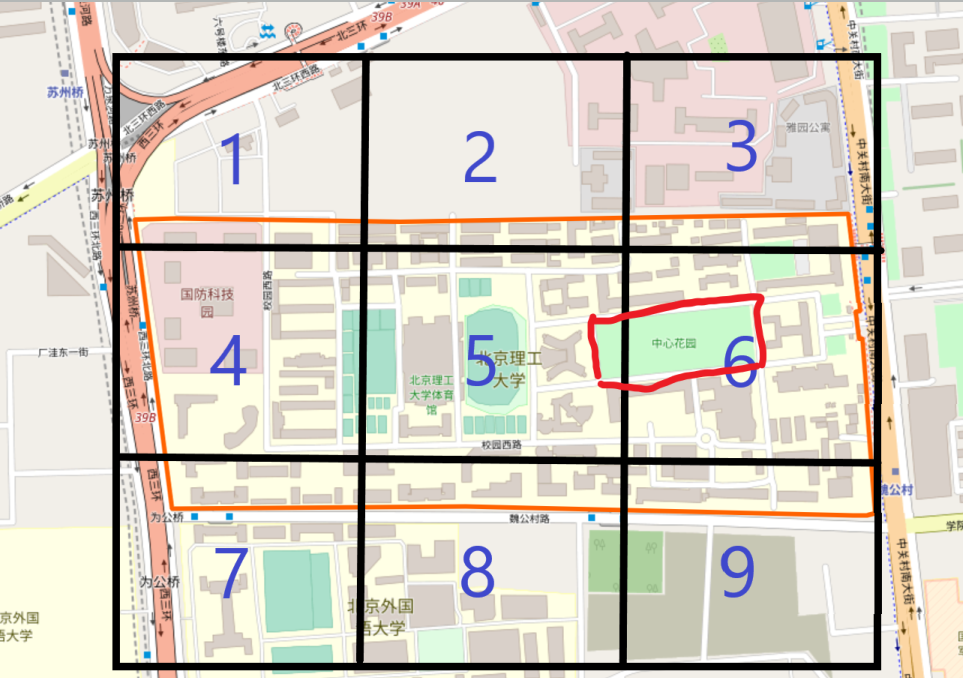
\includegraphics[width=4in]{images/5.png}
    \caption{建筑物绑定区域}\label{建筑物绑定区域} % label 用来在文中索引
  \end{figure}
\subsection{地图存储合约}
合约里面,首先构建了存储一条地图信息的结构体,如图\ref{地图信息结构体}:
\begin{figure}[H]
  \centering
  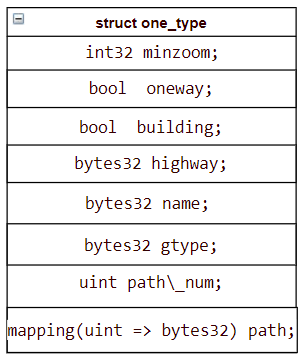
\includegraphics[width=2in]{images/16.png}
  \caption{地图信息结构体}\label{地图信息结构体} % label 用来在文中索引
\end{figure}

对于每条地图数据会有对应的gid编号,通过mapping完成区域与区域内信息的映射。

地图存储合约算法如下:
\begin{algorithm}[H]
  \caption{存储合约} %算法的名字
  \begin{algorithmic}[1] %每行显示行号  
      % \Require Array数组,n数组大小  
      \Require minzoom,oneway,building,highway,name,gtype
      \Function {get\_onetype}{gid}  
        \Return {types\_list[gid]}
      \EndFunction  

      \Function {get\_types}{hash} \\ 
          //获取对应geohash区域内所有道路信息 \\ 
          \Return{geo\_maps[hash]}
      \EndFunction  
      \Function {add\_onetype}{gid,minzoom,oneway,building,highway,name,gtype,path}\\  
          //通过id查询信息
          \State  Onetype.minzoom <- minzoom;
          \State  Onetype.oneway <- oneway;
          \State  Onetype.building <- building;
          \State  Onetype.highway <- highway;
          \State  Onetype.name <-name;
          \State  Onetype.gtype <- gtype;
          \State  Onetype.path <- path;
      \EndFunction  
      \Function {add\_area\_line}{hash,gid}  //绑定区域
          \State num <- geo\_maps[hash].num++;
          \State geo\_maps[hash].types\_list[num] <- gid;
      \EndFunction
  \end{algorithmic}  
\end{algorithm}

\section{小结}
本章中,首先对GeoHash编码进行了介绍,阐明了经纬度数据到GeoHash编码的基本逻辑,并简要介绍GeoHash的相关优点。另外,本章完成了将地图的经纬度数据到GeoHash数据的转换,阐明了地图数据区域绑定的基本逻辑,至此地图存储工作完成,后续将通过GeoHashTile前端结合,展现地图效果。
%%
% The BIThesis Template for Bachelor Graduation Thesis
%
% 北京理工大学毕业设计(论文)第一章节 —— 使用 XeLaTeX 编译
%
% Copyright 2020 Spencer Woo
%
% This work may be distributed and/or modified under the
% conditions of the LaTeX Project Public License, either version 1.3
% of this license or (at your option) any later version.
% The latest version of this license is in
%   http://www.latex-project.org/lppl.txt
% and version 1.3 or later is part of all distributions of LaTeX
% version 2005/12/01 or later.
%
% This work has the LPPL maintenance status maintained'.
%
% The Current Maintainer of this work is Spencer Woo.
%
% 第四章节
\chapter{基于GeoHash的矢量地图展现}
LeafLet\cite{leafletweb}是用于地图的开源JavaScript库之一,它是B / S端WebGIS开发项目中广泛使用的开源软件。开发人员可以基于相关库提供的接口进行开发和扩展,并实现地理信息服务的调用和地图数据的基本操作\cite{edler2019simplicity}。

Leaflet强大的开源库插件涉及地图应用程序的各个方面,包括地图服务,数据提供,数据格式,地理编码,路线搜索,地图控制和交互等,并且还支持自定义控件的实现。这些控件丰富了Leaflet的功能\cite{brambilla2016adgt}。GeoHashTile是基于轻量级的WebGIS库Leaflet来完成GeoHash编码地图数据展现的功能的。

基于地理信息的应用程序,例如导航服务和电子出租车服务为日常生活提供了极大的便利并促进了个人移动设备的普及\cite{li2018bringing},为了获得更好的用户体验,有必要提高访问速度,同时确保有效信息的保留。在“访问速度”和视觉效果之间找到最佳的方法是通过划分、索引和压缩大型地图数据来减少数据传输和提高效率。在大多数文献中,传输的数据元素是携带经纬度坐标的矢量地图数据,如果使用一维字符代表经纬度,这是减少传输数据量的可行方法;另外,对于大多数平铺地图,网络空间索引是被认为是对大量数据访问的有效改进方法,但是,网络空间索引使用三字段查询,这使得在大量数据访问的情况下效率十分低下,第三,数据压缩的数据不会显著降低视觉效果,同时量化方法通过减少位数来压缩数据和实值坐标的精度,可以保持对象的拓扑关系,但是,当实现良好的视觉效果时,如何选择合理的数据量化尺度是一个亟待解决的问题\cite{lawder2000using}。为此,GeoHashTile很好的解决了此类问题。

\section{GeoHashTile简介}
GeoHashTile是基于GeoHash编码的地图数据显示方法,改进了传统地理数据显示在数据索引,数据压缩,以及不同粒度的预测\cite{zhou2020geohashtile}。在此系统中,它使用Geohash编码系统代表坐标,并以此对大型地理数据进行分区和索引,数据压缩和图块编码也由GeoHash完成;它同时采用相对位置投影方法实现在GeoHash和屏幕像素坐标之间的直接转换,最后使用中间结果缓存的方法来提高计算和渲染效率。
\section{GeoHashTile架构}
GeoHashTile系统由两部分组成:服务器端和客户端,服务端提供矢量地理数据服务,客户端完成GeoHash矢量地理数据的显示,包括GeoHashTile计算过程,服务器地图数据的请求过程,GeoHash地图数据的投影过程以及中间结果缓存过程\cite{zhou2020geohashtile}。该功能框架如下:

服务器的工作分为两部分:Geohash矢量地理数据转换和Geohash矢量地理数据服务。数据转换中,将原始GeoJSON数据集的纬度和经度坐标转换为相对应的指定长度的Geohash编码的GeoJSON格式数据,并将数据重新组织为GeoJSON格式数据以供客户端访问,该数据还定义了数据访问接口并设置数据精度。收到客户端发送的HTTP请求后,数据服务部分将分解字段,查询相应的Geohash编码的GeoJSON数据,并通过HTTP响应将其返回给客户端,其中Geohash编码的矢量地理数据服务由GeoServer提供-基于Web的服务器。

客户端工作分为四个部分:
\begin{enumerate}
    \item GeoHashTile计算部分,计算一块GeoHashTile的大小,计算客户端中GeoHashTile的数量,以及计算客户端中所有GeoHashTile编码
    \item 接收地图数据
    \item 通过相对位置投影的方法,实现屏幕像素点到GeoHash坐标值的转换
    \item 通过中间结果缓存来减少重复计算处理,加快图像的呈现
\end{enumerate}

\section{GeoHashTile优点}
GeoHashTile以减少数据传输,提高索引效率和减少加载时间的目标出发,研究了基于GeoHash的矢量地理数据结构,同时提出了地图数据的GeoHashTile系统索引,实现了GeoHash坐标编码的地图数据展示。GeoHashTile系统在减少用户的等待时间的同时不会影响显示效果,它使应用程序减少了数据传输和加载时间,它还提供了支持GeoHash编码的新矢量数据服务,实验结果表明,在减少数据量方面,由于GeoHash压缩了经纬度,不同级别的不同粒度地图数据的存储以及数据合并访问,因此GeoHashTile的平均表现要比GeoTile优43.7\%,web客户端上GeoHashTile的加载时间也比GeoTile短30.2\%。

\section{总体测试框架和运行环境}
\subsection{测试环境}
本次测试,使用nvm-v0.37.2管理nodejs版本,使用npm-v6.14.11包管理,智能合约语言使用Solidty-v0.5.16,在前端调用合约方法上,使用web3js-v1.2.9与之进行交互。在对合约 进行测试时,采用ganache-cli提供本地临时区块链私有链服务,并使用Truffle-v5.1.62辅助部署智能合约,简化了开发和测试流程。在正式应用上,采用geth-v1.9.12以太坊客户端,部署本地私有链,存储相关信息。因为本文应用均是基于最新的开发环境,在编写合约和测试过程中遇到过很多问题,因此编写了许多有关环境配置以及简单示例文件的相关帮助手册,希望能为其他人提供帮助。

\subsection{测试流程}
为了验证地图存储的正确性,本文将此工作与前人相关工作合并,使用GeoHashTile前端对地图数据进行展示。

随着区块链的普遍应用,对应平台也逐渐增多,主流平台还是以太坊。此测试也是在该平台进行相关操作,总体测试流程如下:

\begin{enumerate}
    \item 首先建立Geth私有链;
    \item 通过truffle工具可以简单部署合约到区块链上;
    \item 通过JS脚本将地图数据进行上传及绑定;
    \item 由于时间原因,该测试只是为了验证地图存储的正确性,所以仅上传部分北京数据,并使用GeoHashTile前端对其信息进行展示,结果如图\ref{GeoHashTile展示结果}GeoHashTile展示结果,\ref{放大图}放大图,\ref{缩小图}缩小图。
    \begin{figure}[!htb]
        \centering
        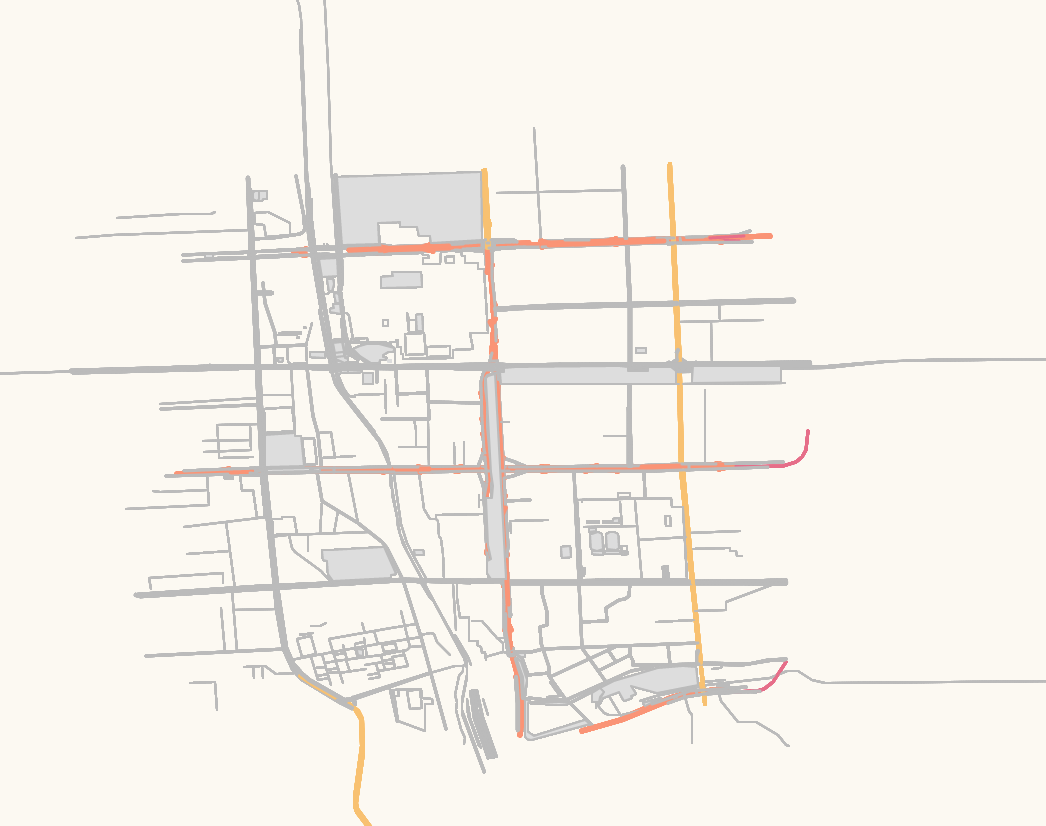
\includegraphics[width=4in]{images/6.png}
        \caption{GeoHashTile展示结果}\label{GeoHashTile展示结果} % label 用来在文中索引
    \end{figure}

    \begin{figure}[!htb]
        \centering
        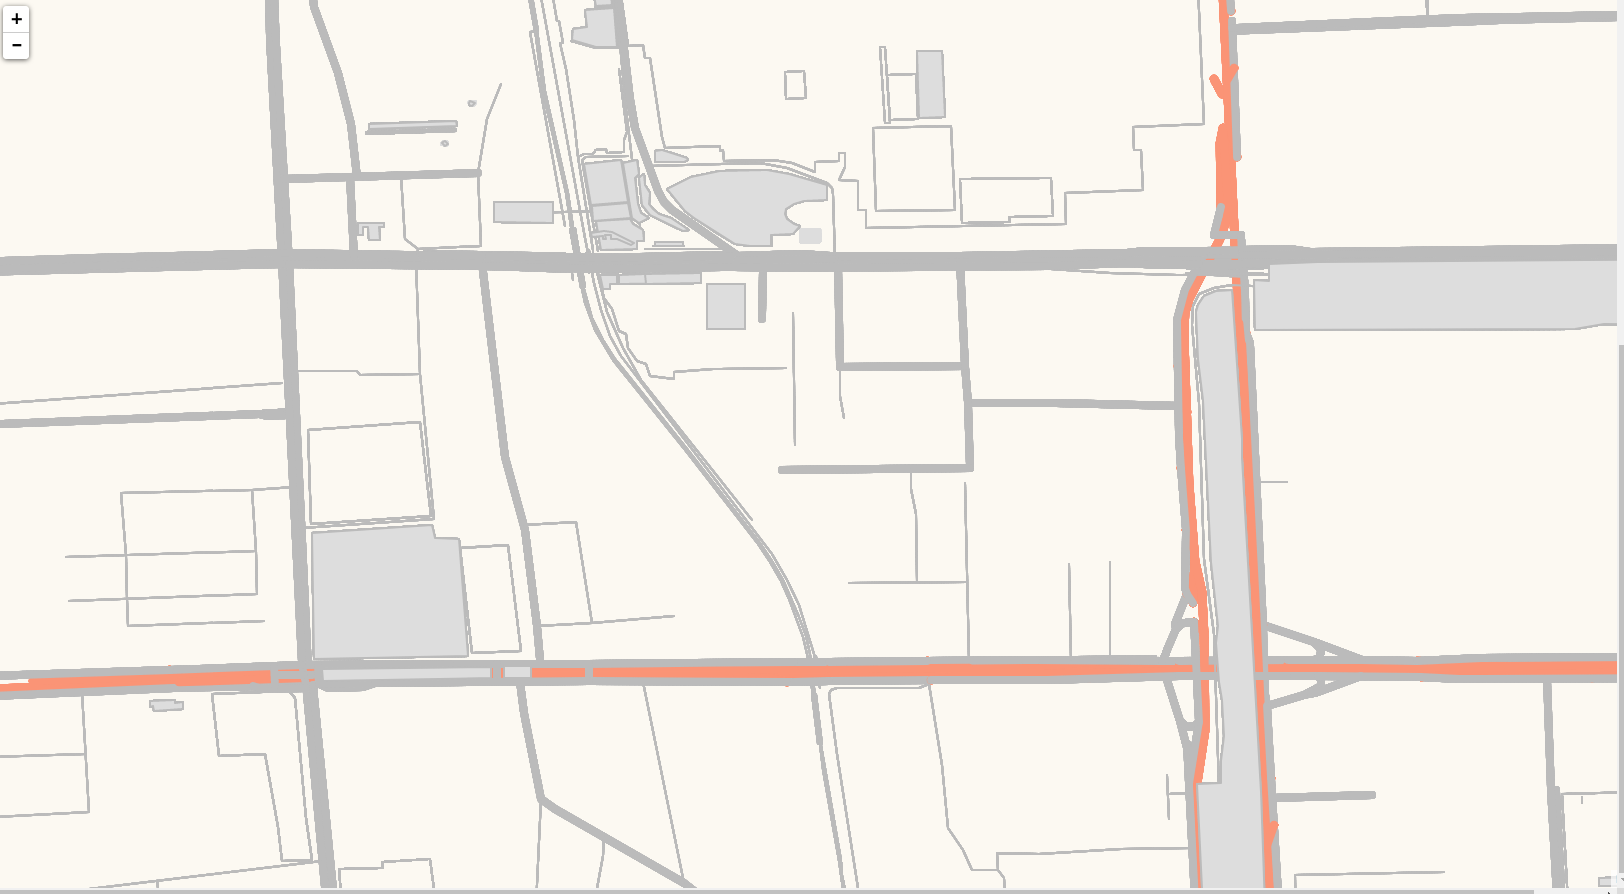
\includegraphics[width=4in]{images/11.png}
        \caption{放大图}\label{放大图} % label 用来在文中索引
    \end{figure}

    \begin{figure}[!htb]
        \centering
        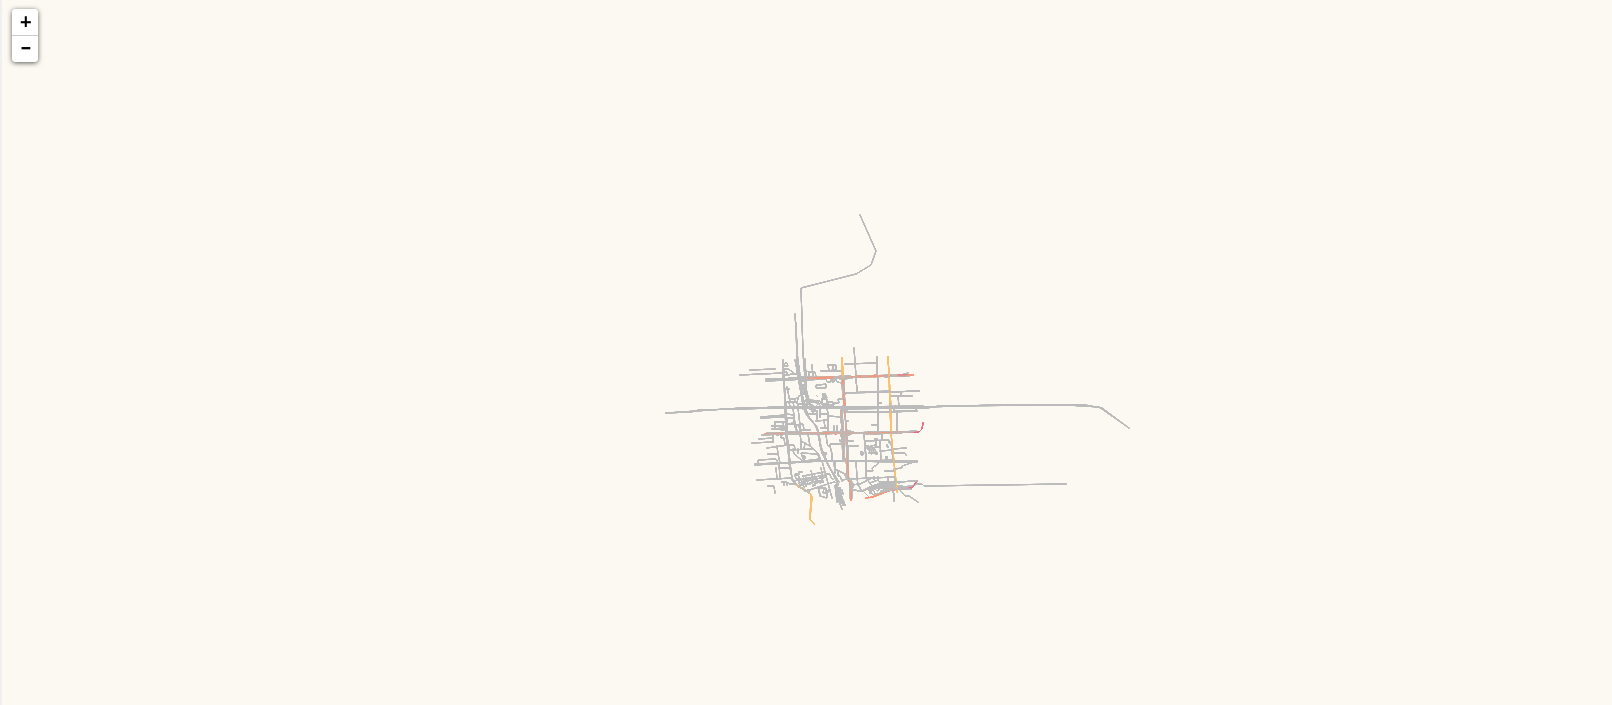
\includegraphics[width=4in]{images/12.png}
        \caption{缩小图}\label{缩小图} % label 用来在文中索引
    \end{figure}
\end{enumerate}

\section{小结}
GeoHash编码使用一维数据替代了二维经纬度数据,同时给地理位置进行了分区,在位数较少时,它可以用来表示某一区域在地球上的坐标,在位数足够时,它也可以用来表示某个具体点在地球上的坐标。在 GeoHash 精度取 8 位的情况下已经可以基本满足代替传统经纬度坐标作为车辆位置精确表示的需求,且若只考虑中国所处纬度(3°51′N 至53°33′N),精度将会提高\cite{lposition}。考虑到车辆位置验证以及道路匹配需要更高的精准度,所以之后的工作中采用了11位长度的GeoHash编码。

GeoHashTile提高了矢量地图的索引效率和加载时间,且提供了支持GeoHash编码的新矢量数据服务。

测试表明,目前该系统可以成功将地图数据经纬度格式转为GeoHash格式,并上传到以太坊私链进行保存,且能够通过GeoHashTile可以正确显示GeoHash矢量数据。
%%
% The BIThesis Template for Bachelor Graduation Thesis
%
% 北京理工大学毕业设计(论文)第一章节 —— 使用 XeLaTeX 编译
%
% Copyright 2020 Spencer Woo
%
% This work may be distributed and/or modified under the
% conditions of the LaTeX Project Public License, either version 1.3
% of this license or (at your option) any later version.
% The latest version of this license is in
%   http://www.latex-project.org/lppl.txt
% and version 1.3 or later is part of all distributions of LaTeX
% version 2005/12/01 or later.
%
% This work has the LPPL maintenance status maintained'.
%
% The Current Maintainer of this work is Spencer Woo.
%
% 第五章节
\chapter{树状区块链应用和性能测试}
本章中,将地图信息存储与展现成功应用于树状区块链上,在此基础上,将李玮琪的车辆位置验证与信誉评估系统\cite{lposition}应用于当前地图存储与显示方法,取得不错的成效。最后,测试了树状区块链与传统区块链存储性能的区别,并得到相关数据结果。

\section{基于区块链地图数据的车辆位置验证与信誉评估系统}
本小节将地图存储与展现工作移植到树状区块链上,并上传北京地图数据,实现了地图展现,在此基础上,复现了李玮琪车辆位置验证与信誉评估\cite{lposition},验证了树状区块链相关功能的正确性。

\subsection{移植地图存储与展现}
首先,根据第一章复现树状区块链的方法建立树状区块链私有链,将地图存储合约进行部署,然后通过JS脚本将北京市地图数据上传,同时进行区域绑定工作。最后,通过GeoHashTile前端将请求获得的数据处理并展现, 结果展示,如图\ref{地图数据上传全图},\ref{局部放大图}。
\begin{figure}[!htb]
    \centering
    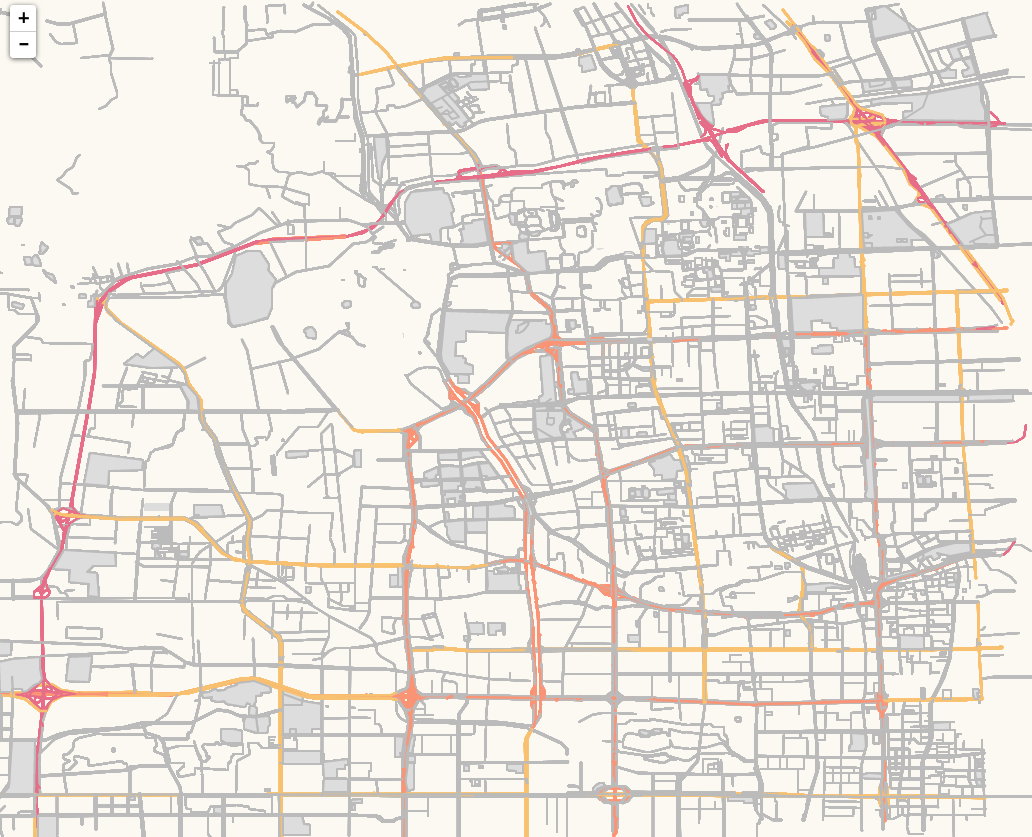
\includegraphics[width=4in]{images/7.png}
    \caption{地图数据上传全图}\label{地图数据上传全图} 
\end{figure}

\begin{figure}[!htb]
    \centering
    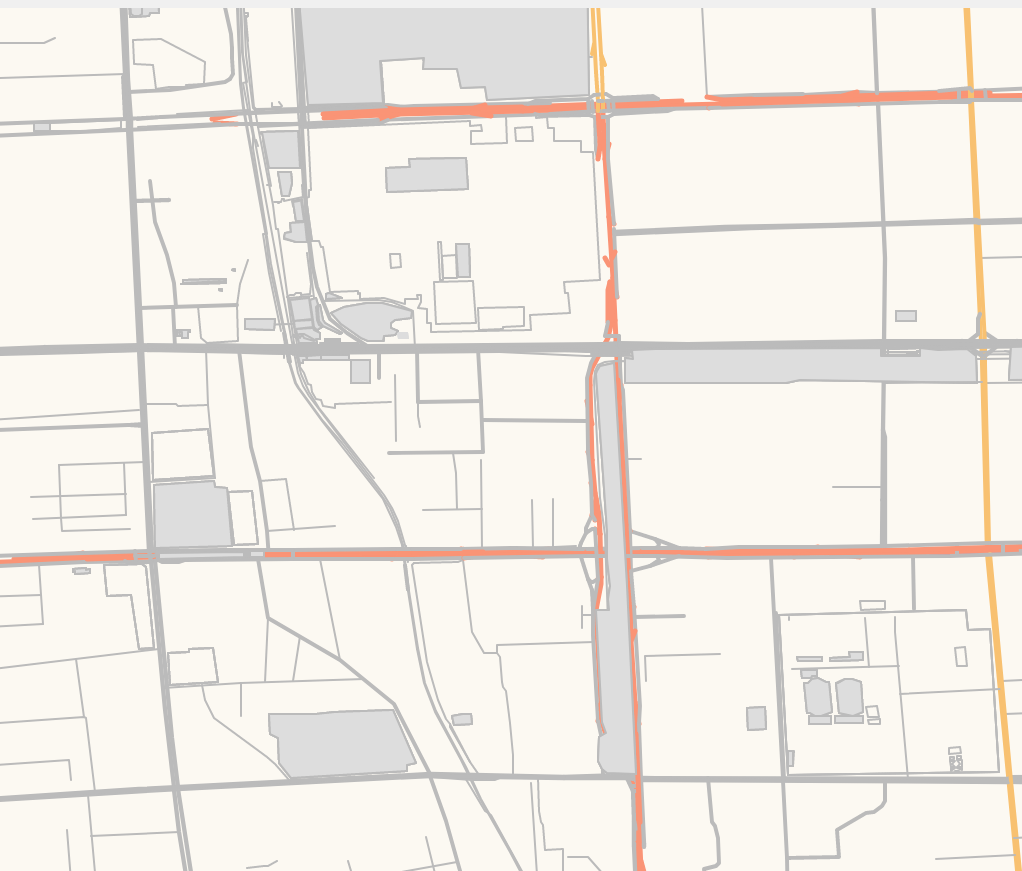
\includegraphics[width=4in]{images/8.png}
    \caption{局部放大图}\label{局部放大图} 
\end{figure}

\subsection{复现车辆位置验证与信誉评估}
车辆位置验证与信誉评估系统,实现了在完成用户验证的基础上为其他使用者提供位置信息和信用评估的数据支持,增强了车载自组网的安全性的同时扩展了应用场景\cite{lposition}。但是,李玮琪调用的地图数据是由openstreetmap提供的矢量地图数据,地图数据安全性得不到保障。本次测试,将李玮琪的工作和地图数据存储和展现结合起来,在完全基于GeoHash编码的GeoHashTile前端进行展示,同时将合约部署至树状区块链上,再次验证树状区块链相关功能的正确性。

车辆位置验证及信誉评估系统主要分为车辆位置采集修正系统和信誉评估系统两个部分\cite{lposition}。车辆位置采集修正系统运行在网页端,获取用户的GPS信息,并根据附近道路实时修正位置,实现与智能合约进行交互,信誉评估系统由只能合约实现并部署在区块链上,负责接收位置采集修正系统的上传的数据,结合已保存的信誉对用户信誉进行更新。

测试流程如下:
\begin{enumerate}
    \item 将信誉评估合约部署至树状区块链上 \\
    由于本文使用的最新的开发环境,重现过程中出现过很多问题,作者对其进行记录,并形成文档,希望对其他人有所帮助。
    \item 将地图显示和该系统结合起来 
    \item 信誉测试路径如图\ref{信誉测试路径}所示
    \begin{figure}[!htb]
        \centering
        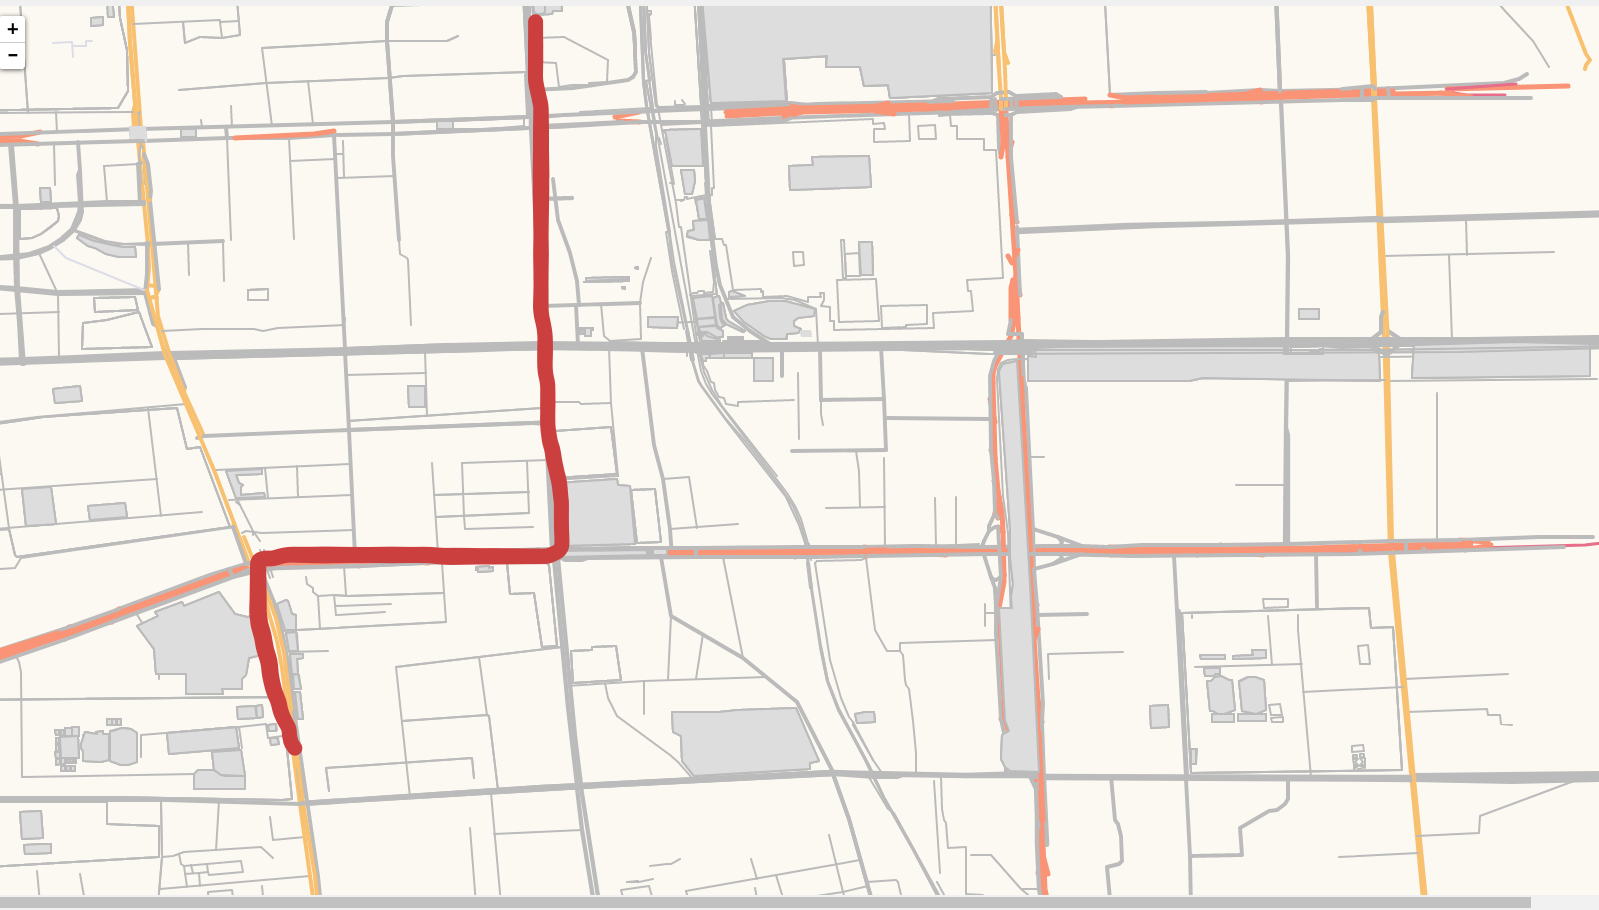
\includegraphics[width=4in]{images/9.png}
        \caption{信誉测试路径}\label{信誉测试路径} 
    \end{figure}

    \item 最终测试结果如图\ref{信誉测试结果}所示
    \begin{figure}[!htb]
        \centering
        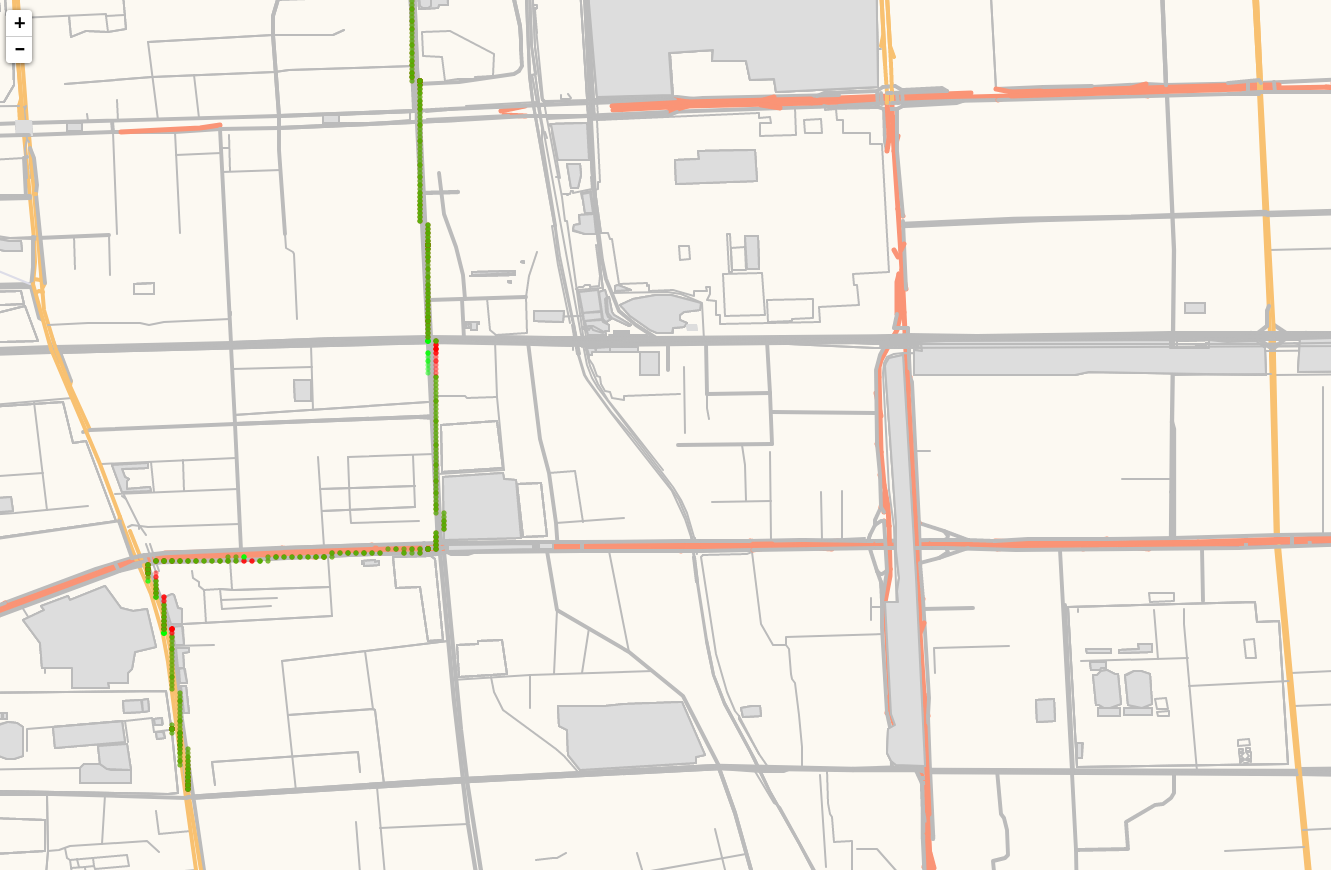
\includegraphics[width=4in]{images/10.png}
        \caption{信誉测试结果}\label{信誉测试结果} 
    \end{figure}
\end{enumerate}

\section{传统区块链合约存储和树状区块链直接存储对比}
此次实验对树状区块链的交易性能进行测试。树状区块链由于本身与地理信息进行绑定,交易时会自动将地理信息存储下来,而传统区块链没有,所以使用智能合约在传统区块链模拟树状区块链的存储状态,对二者效率进行对比,从而评定树状区块链的效率。
\subsection{实验设计思路}
树状区块链会自动维护区域状态树和账户状态树,交易时本身就会存储位置信息。为了在传统区块链上模拟树状区块链的存储量,本次测试需要设计存储合约。

存储合约算法如算法\ref{存储合约}。
\begin{algorithm}[t]
    \caption{存储合约} %算法的名字
    \label{存储合约}
    \begin{algorithmic}[1] %每行显示行号  
        % \Require Array数组,n数组大小  
        \Require from\_account,position,transactionhash,receipt,txttime
        \Function {setInfo}{from\_account,position,transactionhash,receipt,txttime} 
            // 实现存储  
            \State  Onelog.from\_account <- from\_account;
            \State  Onelog.position <- position;
            \State  Onelog.transactionhash <- transactionhash;
            \State  Onelog.recleipt <- receipt;
            \State  Onelog.txttime <-txttime;
            \State  bind\_to\_position(position,from\_account)
        \EndFunction  

        \Function {bind\_to\_position}{position,from\_account}  //实现位置绑定 
            //去重
            \If {CheckDup(from\_account)} 
            {
                \Return
            }
            \Else
                \State position\_area\_accounts[position].num <- position\_area\_accounts[position].num + 1;
                \State position\_area\_accounts[position].account\_list[num] <- from\_account
            \EndIf
        \EndFunction  
        \Function {getInfo\_by\_id}{id}  //通过id查询信息
            \Return {from\_account,position,transactionhash,receipt,txttime}
        \EndFunction  
        \Function {getAccount\_by\_position}{position}  //通过位置查询信息
            \State accounts <- NULL
            \State length <-  position\_area\_accounts[position].num;
            \For {i = 0 -> length}
                \State accounts[i] = position\_area\_accounts[position].account\_list[i]
            \EndFor 
            \Return accounts;
        \EndFunction
    \end{algorithmic}  
\end{algorithm}

本次测试中,传统区块链和树状区块链实际存储数据内容相同,传统区块链由于没有与位置信息进行绑定,所以采用合约的方法进行存储,模拟树状区块链状态,而树状区块链则采用eth直接发送交易,测试算法如算法\ref{测试算法}。
\begin{algorithm}[t]
    \caption{测试算法} %算法的名字
    \label{测试算法}
    \begin{algorithmic}[1] %每行显示行号  
       \State web3绑定
       \State spos1 <- "w1111111111111";
       \State st <- Date();
       \For{i = 0 -> length}
            \State si = i.toString()
            \State subpos <- spos1.substr(0,14-sj.length);
            \State \_position <- subpos+sj;
            \State 合约交易或eth.sendtransaction直接交易
            \State sleep(100);
       \EndFor
       \State 等待区块链存储完毕
       \State se <- Date()-st
       \State 打印结果
    \end{algorithmic}  
\end{algorithm}
\subsection{实验结果}
\begin{table}[!ht]
    \centering
    \caption{测试结果}
    \label{测试结果}
    \begin{tabular}{*{4}{>{\centering\arraybackslash}p{3cm}}}
    \hline
           &  存储数据量      & 传统区块链合约存储时间        & 树状区块链直接存储时间      \\ \hline
      1    &  1200条         & 179518ms                    & 179888ms                  \\
      2    &  2400条         & 376738ms                    & 358368ms                  \\
      3    &  6000条         & 952859ms                    & 915299ms                  \\ 
      4    &  12000条        & 1871136ms                   & 1812014ms                  \\
      \hline
      \end{tabular}
  \end{table}

  表\ref{测试结果}中显示,同样的数据量存储,利用智能合约存储至传统区块链中要比树状区块链直接存储的时间长,而且,这种趋势将随着这数据量的增多而愈发明显。根据上述数据对比,树状区块链对于信息存储效率要比传统区块链好,且树状区块链自身与位置信息绑定,又提供区域查询等更多位置信息查询功能,要比传统区块链更适应于车载自组网。

  \section{小结}
本章中,在树状区块链和地图存储的基础上复现了李玮琪的车辆位置验证与信誉评估的工作,验证了树状区块链的正确性。最后,对树状区块链存储方面进行了性能测试,可以明显发现,随着发送数量的增加,树状区块链本身具备地理信息的优势逐渐增大,存储速率要比传统区块链有所加快,并随着数据量的增加而越发明显,树状区块链在存储同样信息的同时,又保证区域绑定、区域查询功能,且能够自动维护区域状态树以及账户状态树,其功能性更加强大。

% 结论:在结论相应的 TeX 文件处进行结论部分的撰写
%%
% The BIThesis Template for Bachelor Graduation Thesis
%
% 北京理工大学毕业设计(论文)结论 —— 使用 XeLaTeX 编译
%
% Copyright 2020 Spencer Woo
%
% This work may be distributed and/or modified under the
% conditions of the LaTeX Project Public License, either version 1.3
% of this license or (at your option) any later version.
% The latest version of this license is in
%   http://www.latex-project.org/lppl.txt
% and version 1.3 or later is part of all distributions of LaTeX
% version 2005/12/01 or later.
%
% This work has the LPPL maintenance status `maintained'.
%
% The Current Maintainer of this work is Spencer Woo.
%
% Compile with: xelatex -> biber -> xelatex -> xelatex

\unnumchapter{结~~~~论}
\renewcommand{\thechapter}{结论}

\ctexset{
  section/number = \arabic{section}
}

% 结论部分尽量不使用 \subsection 二级标题,只使用 \section 一级标题
智能汽车的广泛使用,使得车辆之间的联系将会越来越紧密,车辆之间的大量信息,使得车载自组网的应用成为可能。利用车载自组网,将智能车辆组织起来,分享和传递数据。车载自组网需要建立去中心化的ad-hoc网络,而区块链具备去中心化、不可篡改、共识机制等特点,所以将区块链技术用于车载自组网中是一种可行方案。然而,车载自组网需要与地理信息密切结合且节点具备移动性特点,但传统区块链的单链结构并不能够很好的解决上述问题。另外,车载自组网的大量应用都与地理位置信息密切相关,而数据来源于开放的互联网平台,存在被篡改的风险,且传统的地理信息以经纬度的形式在矢量地图表示,在区域信息绑定、信息安全等问题上存在问题。

针对上述问题,本文完成了对区块链多链结构的相关调研,并对树状区块链相关工作进行了介绍,同时在此基础上对当前工作完成了复现。同时,作者对地图信息存储和展现进行了相关研究,并最终实现了基于GeoHash编码的地图信息存储,同时结合区块链的不可篡改特性,保证了地图数据可靠性,并最终通过基于LeafLet的轻量级GeoHashTile前端展现最终的矢量地图,实现了完全基于GeoHash编码的存储和展现,利用GeoHash编码特性,简化了地图存储绑定逻辑,同时减小了请求传递的数量级别,对地图存储展现有所推进。

另外,本文最后一章,对树状区块链进行了相关验证和测试,成功解决合约部署问题,将地图存储和展现的全部工作移植到树状区块链上,同时成功应用了李玮琪的车辆位置验证与信誉评估系统,验证了树状区块链功能的正确性。同时,设计了相关实验和算法,对树状区块链的相关性能进行了测试,在相同的数据存储下,树状区块链会快于传统区块链,同时此结果将随着数据量增多而愈发明显。
% 参考文献:如无特殊需要,参考文献相应的 TeX 文件无需改动,添加参考文献请使用 BibTeX 的格式
%   添加至 misc/ref.bib 中,并在正文的相应位置使用 \cite{xxx} 的格式引用参考文献
%%
% The BIThesis Template for Bachelor Graduation Thesis
%
% 北京理工大学毕业设计(论文)参考文献 —— 使用 XeLaTeX 编译
%
% Copyright 2020 Spencer Woo
%
% This work may be distributed and/or modified under the
% conditions of the LaTeX Project Public License, either version 1.3
% of this license or (at your option) any later version.
% The latest version of this license is in
%   http://www.latex-project.org/lppl.txt
% and version 1.3 or later is part of all distributions of LaTeX
% version 2005/12/01 or later.
%
% This work has the LPPL maintenance status `maintained'.
%
% The Current Maintainer of this work is Spencer Woo.
%
% Compile with: xelatex -> biber -> xelatex -> xelatex
%
% 如无特殊需要,本页面无需更改

% 参考文献开始
\unnumchapter{参考文献}
\renewcommand{\thechapter}{参考文献}

% 设置参考文献字号为 5 号
\renewcommand*{\bibfont}{\zihao{5}}
% 设置参考文献各个项目之间的垂直距离为 0
\setlength{\bibitemsep}{0ex}
\setlength{\bibnamesep}{0ex}
\setlength{\bibinitsep}{0ex}
% 设置单倍行距
\renewcommand{\baselinestretch}{1.2}
% 设置参考文献顺序标签 `[1]` 与文献内容 `作者. 文献标题...` 的间距
\setlength{\biblabelsep}{0.5mm}
% 设置参考文献后文缩进为 0(与 Word 模板保持一致)
\renewcommand{\itemcmd}{
  \addvspace{\bibitemsep} % 恢复 \bibitemsep 的作用
  \mkgbnumlabel{\printfield{labelnumber}}
  \hspace{\biblabelsep}}
% 删除默认的「参考文献 / Reference」标题,使用上面定义的 section 标题
% 在使用时,请删除/注释上方示例内容,并启用下方语句以输出所有的参考文献
\printbibliography[heading=none]
% 附录:在附录相应的 TeX 文件处进行附录部分的撰写
%%
% The BIThesis Template for Bachelor Graduation Thesis
%
% 北京理工大学毕业设计(论文)附录 —— 使用 XeLaTeX 编译
%
% Copyright 2020 Spencer Woo
%
% This work may be distributed and/or modified under the
% conditions of the LaTeX Project Public License, either version 1.3
% of this license or (at your option) any later version.
% The latest version of this license is in
%   http://www.latex-project.org/lppl.txt
% and version 1.3 or later is part of all distributions of LaTeX
% version 2005/12/01 or later.
%
% This work has the LPPL maintenance status `maintained'.
%
% The Current Maintainer of this work is Spencer Woo.
%
% Compile with: xelatex -> biber -> xelatex -> xelatex

\unnumchapter{附~~~~录}
\renewcommand{\thechapter}{附录}

% 设置附录编号格式
\ctexset{
  section/number = 附录\Alph{section}
}

% 这里示范一下添加多个附录的方法:

\section{传统区块链私有链建立}
\begin{enumerate}
  \item 建立私链首先需要构建创世块,如下是本课题传统区块链上所使用的创世块genesis.json 
  \begin{center}
    \fbox{
      \parbox{130mm}{
        \{
            "config": \{ \\
            "chainId": 666,
            "homesteadBlock": 0, 
            "eip150Block": 0, \\
            "eip150Hash": "0x0000000000000000000000000000000000000000000000 \par 000000000000000000",\\
            "eip155Block": 0, 
            "eip158Block": 0, 
            "byzantiumBlock": 0, \\
            "constantinopleBlock": 0,
            "petersburgBlock": 0,
            "istanbulBlock": 0,\\
            "ethash": \{\}
        \},
        "nonce": "0x0",
        "timestamp": "0x5ddf8f3e",\\
        "extraData": "0x00000000000000000000000000000000000000000000 \par 00000000000000000000",\\
        "gasLimit": "0x47b760", 
        "difficulty": "0x00002",\\
        "mixHash": "0x000000000000000000000000000000000000000000000000 \par 0000000000000000", \\
        "coinbase": "0x0000000000000000000000000000000000000000",\\
        "alloc": \{ \}, 
        "number": "0x0",
        "gasUsed": "0x0",\\
        "parentHash": "0x00000000000000000000000000000000000000000000000 \par 00000000000000000"
        \}
      }
    }
  \end{center}
  \item 初始化私链
  \begin{center}
    \fbox{
        geth init ./genesis.json --datadir "./chain"
    }
  \end{center} 
  之后所有私链上的相关信息都将保存至chain文件夹中
  \item 启动私链 
  \begin{center}
    \fbox{
        \parbox{130mm}{
            geth --identity "etherum" --rpcaddr 127.0.0.1 --rpc --rpcport "8545" --rpccorsdomain "*"  --maxpeers 2 --rpcapi "personal,eth,net,web3,debug" --networkid 100 --datadir "./chain" --nodiscover --allow-insecure-unlock --dev.period 1 console
        }
    }
\end{center} 
由于GeoHashTile前端使用html编写,通过web3与合约进行交互,为此,需要开启rpc选项,并指定对应端口,才能正确访问合约。
\end{enumerate}
        
   

\section{Truffle合约编译与部署}
\begin{enumerate}
  \item 新建文件夹并初始化;
  \begin{center}
    \fbox{
      \parbox{130mm}{
        mkdir test \\
        truffle init
      }
    }
  \end{center}
  \item 在contracts文件夹中添加合约StoreTraffic.sol;
  \item 在migrations文件夹中添加部署文件; \\
  注意:变量名开头需要大写,且与合约文件名一致。
  \begin{center}
    \fbox{
        \parbox{130mm}{
          const StoreTraffic = artifacts.require("StoreTraffic");\\
          module.exports = function(deployer) \{ \\
            deployer.deploy(StoreTraffic); \\
          \};          
        }
    }
\end{center} 
  \item 更改truffle-config.js文件,监控本地网络;
  \begin{center}
    \fbox{
        \parbox{130mm}{
          module.exports = \{ \\
          networks: \{ \\
            development: \{ \\
              host: "localhost", \\
              port: 8545, \\
              network\_id: "*" // Match any network id \\
            \} 
          \}
        \};
          
        }
    }
\end{center} 
  \item truffle compile 编译合约
  \item truffle migrate 部署合约
\end{enumerate}

\section{树状区块链私有链创世块}
\begin{center}
  \fbox{
    \parbox{130mm}{
      \{ \\
      "config": \{ 
      "chainId": 91036, 
      "homesteadBlock": 0, 
          "eip150Block": 0, 
          "eip155Block": 0, \\
          "eip158Block": 0, 
          "byzantiumBlock": 0,  
          "constantinopleBlock": 0, 
          "petersburgBlock": 0 \\
        \},
        "alloc": \{
        \}, \\
        "coinbase": "0x0000000000000000000000000000000000000000",\\
        "difficulty": "0x20000", \\
        "extraData": "", \\
        "gasLimit": "0xffffffff", \\
        "nonce": "0x0000000000000042", \\
        "mixhash": "0x00000000000000000000000000000000000000000000 \par 00000000000000000000", \\
        "parentHash": "0x0000000000000000000000000000000000000000000 \par 000000000000000000000", \\
        "timestamp": "0x00" \\
      \}
    }
  }
\end{center}
% 致谢:在致谢相应的 TeX 文件处进行致谢部分的撰写
%%
% The BIThesis Template for Bachelor Graduation Thesis
%
% 北京理工大学毕业设计(论文)致谢 —— 使用 XeLaTeX 编译
%
% Copyright 2020 Spencer Woo
%
% This work may be distributed and/or modified under the
% conditions of the LaTeX Project Public License, either version 1.3
% of this license or (at your option) any later version.
% The latest version of this license is in
%   http://www.latex-project.org/lppl.txt
% and version 1.3 or later is part of all distributions of LaTeX
% version 2005/12/01 or later.
%
% This work has the LPPL maintenance status `maintained'.
%
% The Current Maintainer of this work is Spencer Woo.
%
% Compile with: xelatex -> biber -> xelatex -> xelatex

\unnumchapter{致~~~~谢}
\renewcommand{\thechapter}{致谢}

\ctexset{
  section/number = \arabic{section}
}

% 致谢部分尽量不使用 \subsection 二级标题,只使用 \section 一级标题

值此论文完成之际,首先向我的导师……

\textcolor{blue}{致谢正文样式与文章正文相同:宋体、小四;行距:22 磅;间距段前段后均为 0 行。阅后删除此段。}



\end{document}